% Created 2019-09-16 Mon 12:00
% Intended LaTeX compiler: pdflatex
\documentclass[10pt,t]{beamer}
\usepackage[utf8]{inputenc}
\usepackage[T1]{fontenc}
\usepackage{graphicx}
\usepackage{grffile}
\usepackage{longtable}
\usepackage{wrapfig}
\usepackage{rotating}
\usepackage{amsmath}
\usepackage{textcomp}
\usepackage{amssymb}
\usepackage{capt-of}
\usepackage{hyperref}
\usetheme{default}
\author{L. Larrabee Strow}
\date{\today}
\title{\large All-Sky AIRS Anomaly Retrievals \newline
  using Zonally Gridded, Time Averaged \newline
  Brightness Temperature Spectra}
\subtitle{\footnotesize{AIRS Science Team Meeting}}
\date{\vspace{0.1in}\footnotesize{September 25, 2019 \vfill}}
\author{Sergio DeSouza--Machado\inst{1,2}, L. Larrabee Strow\inst{1,2}}
\institute[UMBC]{\inst{1} UMBC Physics Dept. \and \inst{2}UMBC JCET}
\input beamer_setup
\usetheme{metropolis}
\metroset{titleformat title=allcaps}
\renewcommand{\UrlFont}{\small\tt}
\renewcommand*{\UrlFont}{\footnotesize}
\tolerance=1000
\RequirePackage{fancyvrb}
\DefineVerbatimEnvironment{verbatim}{Verbatim}{fontsize=\footnotesize}
\begin{document}

\maketitle
\addtobeamertemplate{block begin}{
  \setlength{\parsep}{0pt}
  \setlength{\topsep}{3pt plus 2pt minus 2.5pt}
  \setlength{\itemsep}{0pt plus 0pt minus 2pt}
  \setlength{\partopsep}{2pt}
}

%anom_noise = load('btn_avg.mat');
%load /home/sbuczko1/git/rtp_prod2/airs/static/f_default_l1c.mat
%plot(f,squeeze(anom_noise.btn_avg(20,:,:))')

\section{Overview}
\begin{frame}
  \frametitle{Overview of talk}
  \begin{itemize}
  \item \textcolor{red}{Larrabee's talk establishes high stability of AIRS(LW/MW)}
  \begin{itemize}
    \item we used noise covariance based on <NedT> per latitude bin \newline 
     ($\le$ 0.001 K at 1231 \wn, tropical latbins) 
    \item instead of using SARTA jacobians for anomalies, we used kCARTA with latest spectroscopy
    (LBLRTM 12.8 for CO2,CH4), HITRAN 2016 for other gases, CKD 3.2
    \item plus we also know kCARTA jacobians work fine for any CO2/T combinations
    \item Clear Sky scenes have very poor global sampling eg concentrated in Arabian Sea
    \item (trace gases uniformly mixed so we retrieve those rates very well)
  \end{itemize}
  \item Using lessons learned from clear sky spectral anomaly and rate retrievals 
     we are now beginning to work with  allsky spectral anomalies and trends.
  \end{itemize}
\end{frame}

\begin{frame}
  \frametitle{Overview of talk (cont'd)}
  \begin{itemize}
  \item kCARTA can do very similar TwoSlab calcs to SARTA, so no problems using it for allsky
        T/WV/O3,surftemp jacobians; for this talk we use SARTA for cloud jacobians
  \item In this talk we work with zonally averaged anomalies
  \item Long term goal is gridded anomalies, and trends derived from those anomalies
  \item We also plan to do an ``onion peeling'' where we use BT1231
    observed and ERA surface temperaure to partition data into
    clear/partly cloudy/very cloudy/DCC; start the retrievals with
    clear and then move upwards (weighting the retrievals with nuber
    of points)
  \item Here we work only with AIRS for proof of principle, plan to do this with CHIRP
  \end{itemize}
\end{frame}

% ---------------------------------------------------------------------
\section{Clear Sky vs ERA Anomalies}
\begin{frame}
  \frametitle{Clear Sky Retrievals}
  \begin{itemize}
    \item Larrabee's talk gives details (data from 2002/09 to 2018/08)
      \begin{itemize}
        \item 16 years of data divided into 16 day averages $\rightarrow$ 365 timesteps
        \item \textcolor{red}{AIRS observations sampled for CLEAR scenes in these bins}
        \item binned into 40 equal area latitude bins (thinner in equator/thicker at polar regions)
        \item BT anomalies and average ERA profiles for all 365 timesteps
      \end{itemize}
    \item kCARTA 97 layer analytic jacobians for surface temperature, T(z), WV(z),O3(z)
    \item Ran off kCARTA at t=0 to t=T to make ``finite difference'' column trace gas jacobians
          (CO2,N2O,CH4,CFC11,CFC12)
    \item Using these jacobians, we retrieved T(t,z), WV(t,z), O3(t,z), CO2(t), N2O(t), CH4(t), 
          CFC11(t), CFC12(t), surftemp(t)
          at each of the 40 latbins $\times $ 365 timesteps
  \end{itemize}
\end{frame}

%%%%%%%%%%%%%%%%%%%%%%%%%

\begin{frame}{Tropical Clear Sky Geophysical Anomalies : T(z,t)}
%% see /home/sergio/MATLABCODE/oem_pkg_run_sergio_AuxJacs/MakeProfs/plot_anomalies.m
\vspace{-0.35in}

\begin{columns}
\begin{column}{0.45\columnwidth}
\begin{block}{\footnotesize ERA}
\vspace{-0.1in}
\begin{center}
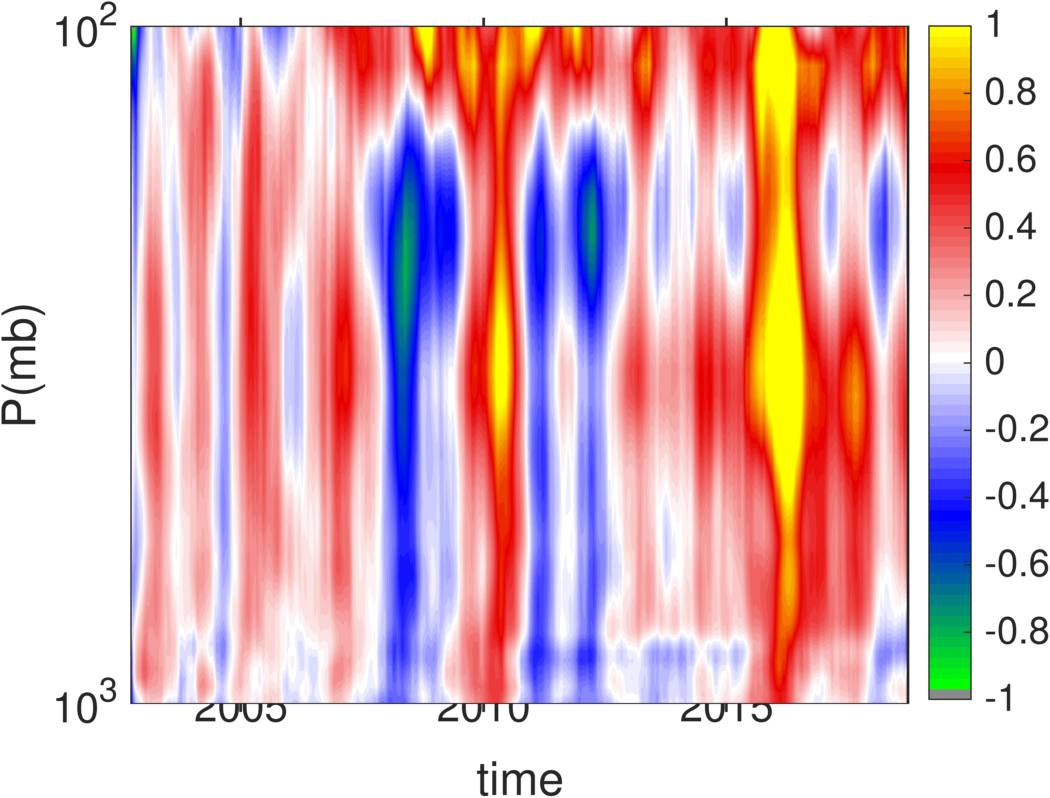
\includegraphics[width=\linewidth]{Figs/ClearAnom/era_clr_ptemp_anom_200209_201808.png}
\end{center}
\end{block}
\end{column}

\begin{column}{0.45\columnwidth}
\begin{block}{}
UMBC Retr Calc are retrievals from simulated radiances derived from ERA.
\end{block}
\end{column}
\end{columns}

\vspace{-0.25in}

\begin{columns}
\begin{column}{0.45\columnwidth}
\begin{block}{\footnotesize UMBC Retr Obs}
\vspace{-0.1in}
\begin{center}
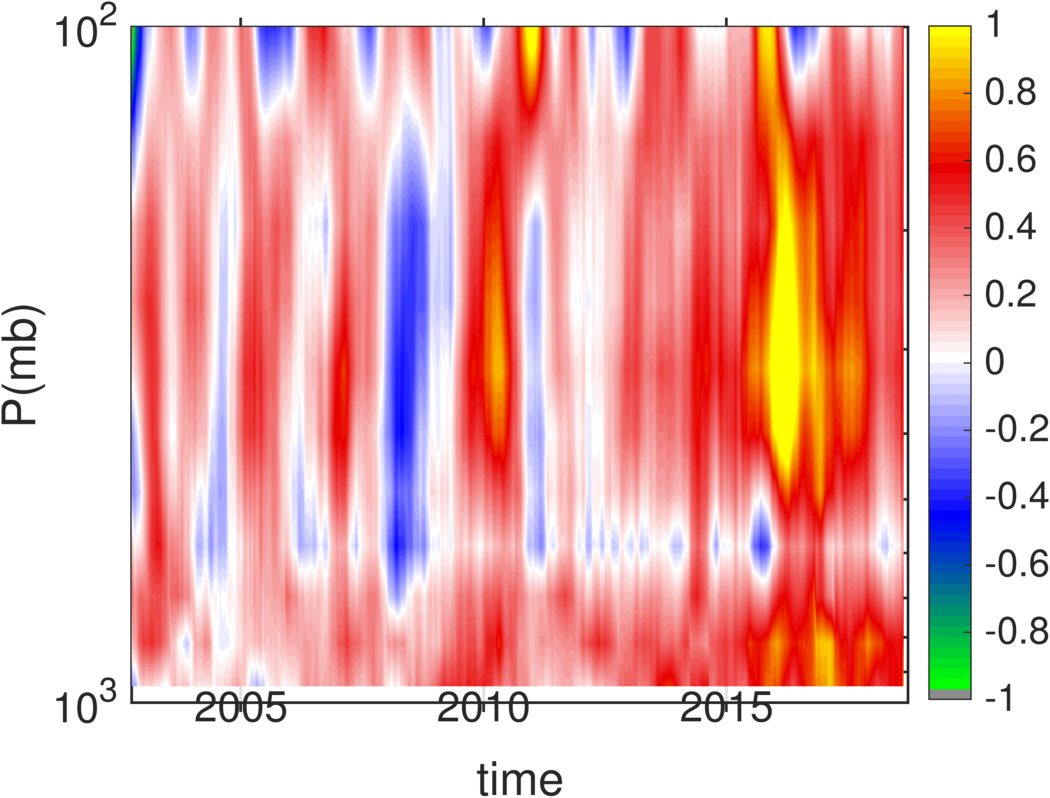
\includegraphics[width=\linewidth]{Figs/ClearAnom/umbc_clr_retr_obs_ptemp_anom_200209_201808.png}
\end{center}
\end{block}
\end{column}

\begin{column}{0.45\columnwidth}
\begin{block}{\footnotesize UMBC Retr Calc}
\vspace{-0.1in}
\begin{center}
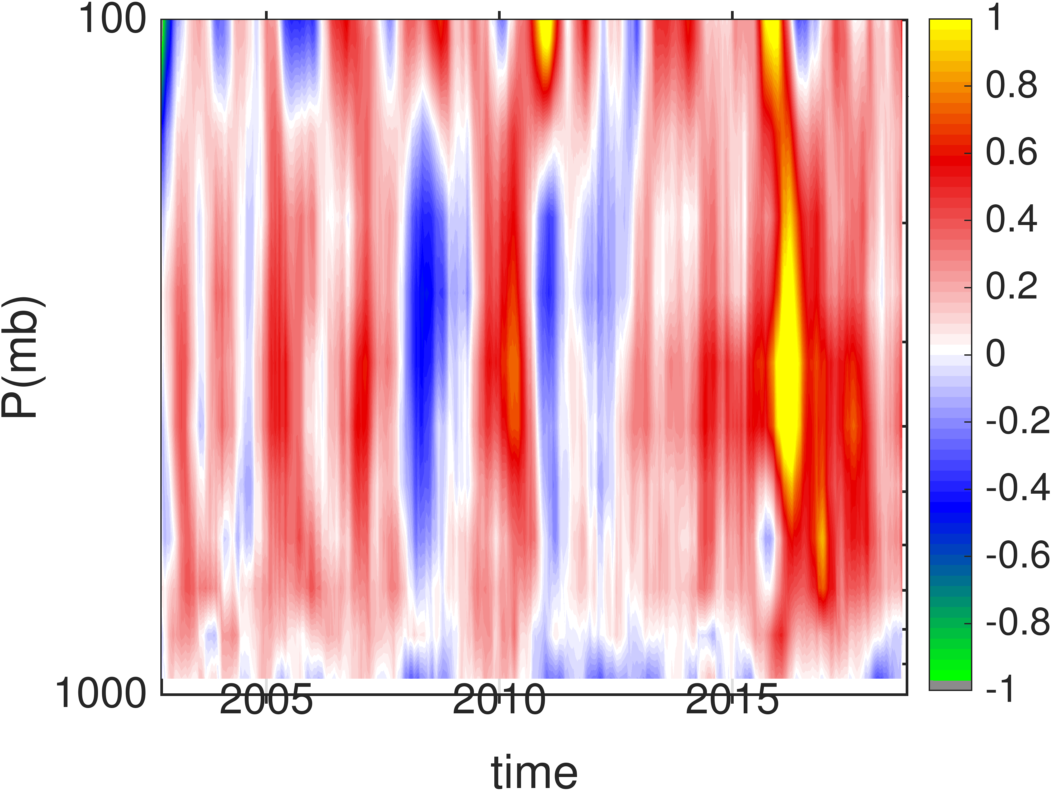
\includegraphics[width=\linewidth]{Figs/ClearAnom/umbc_clr_retr_cal_ptemp_anom_200209_201808.png}
\end{center}
\end{block}
\end{column}
\end{columns}

\end{frame}

%%%%%%%%%%%%%%%%%%%%%%%%%

\begin{frame}{Tropical Clear Sky Geophysical Anomalies : \textit{frac} WV(z,t)}
%% see /home/sergio/MATLABCODE/oem_pkg_run_sergio_AuxJacs/MakeProfs/plot_anomalies.m
\vspace{-0.35in}

\begin{columns}
\begin{column}{0.45\columnwidth}
\begin{block}{\footnotesize ERA}
\vspace{-0.1in}
\begin{center}
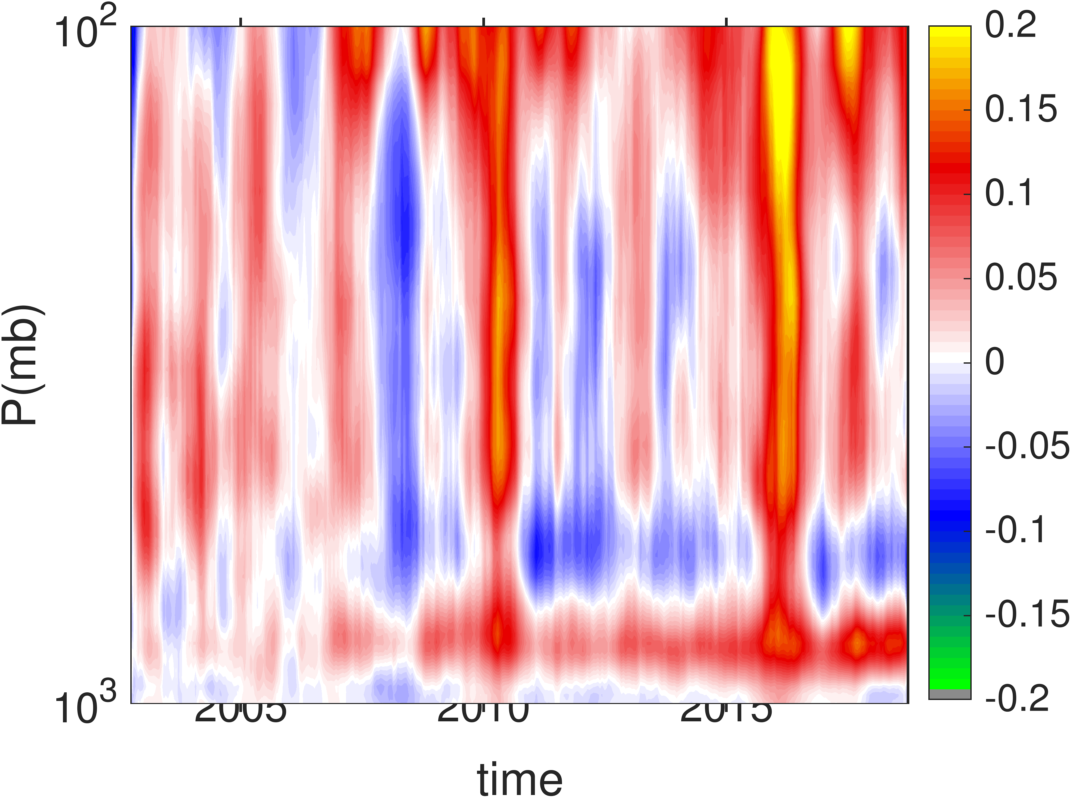
\includegraphics[width=\linewidth]{Figs/ClearAnom/era_clr_wv_anom_200209_201808.png}
\end{center}
\end{block}
\end{column}

\begin{column}{0.45\columnwidth}
%\begin{block}{\footnotesize $frac$ WV(z,t)}
%\vspace{-0.1in}
%\begin{center}
%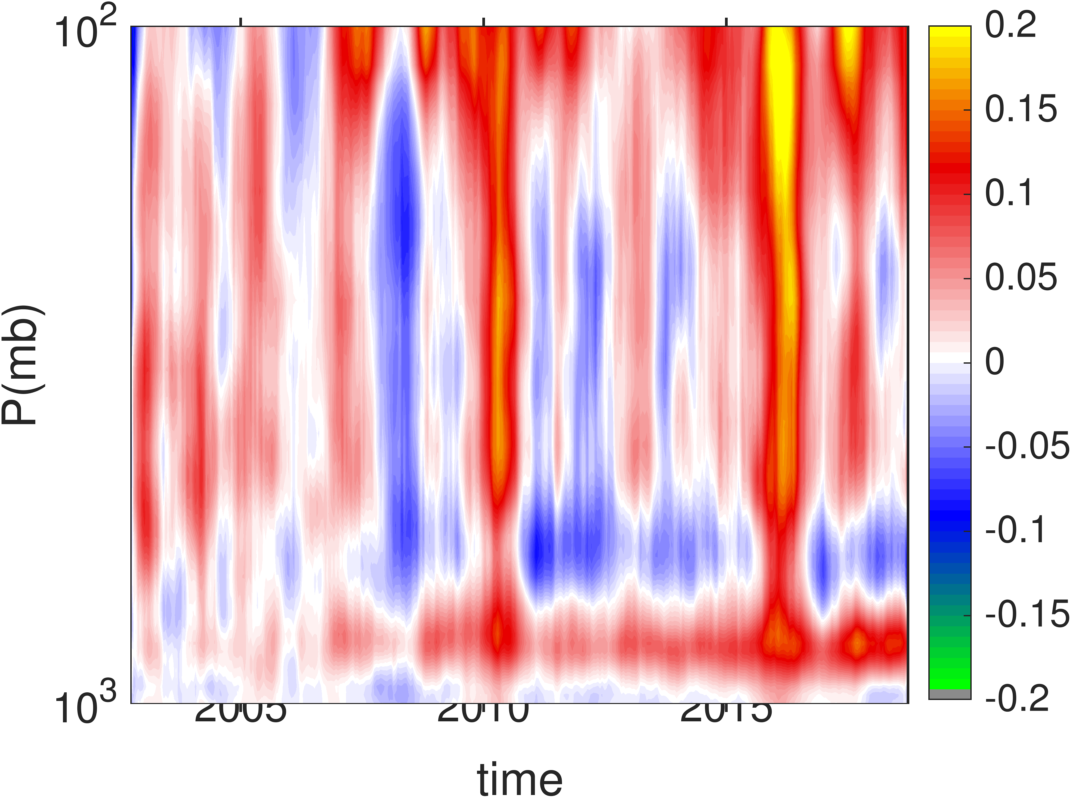
\includegraphics[width=\linewidth]{Figs/ClearAnom/era_clr_wv_anom_200209_201808.png}
%\end{center}
%\end{block}
\end{column}
\end{columns}

\vspace{-0.25in}

\begin{columns}
\begin{column}{0.45\columnwidth}
\begin{block}{\footnotesize UMBC Retr Obs}
\vspace{-0.1in}
\begin{center}
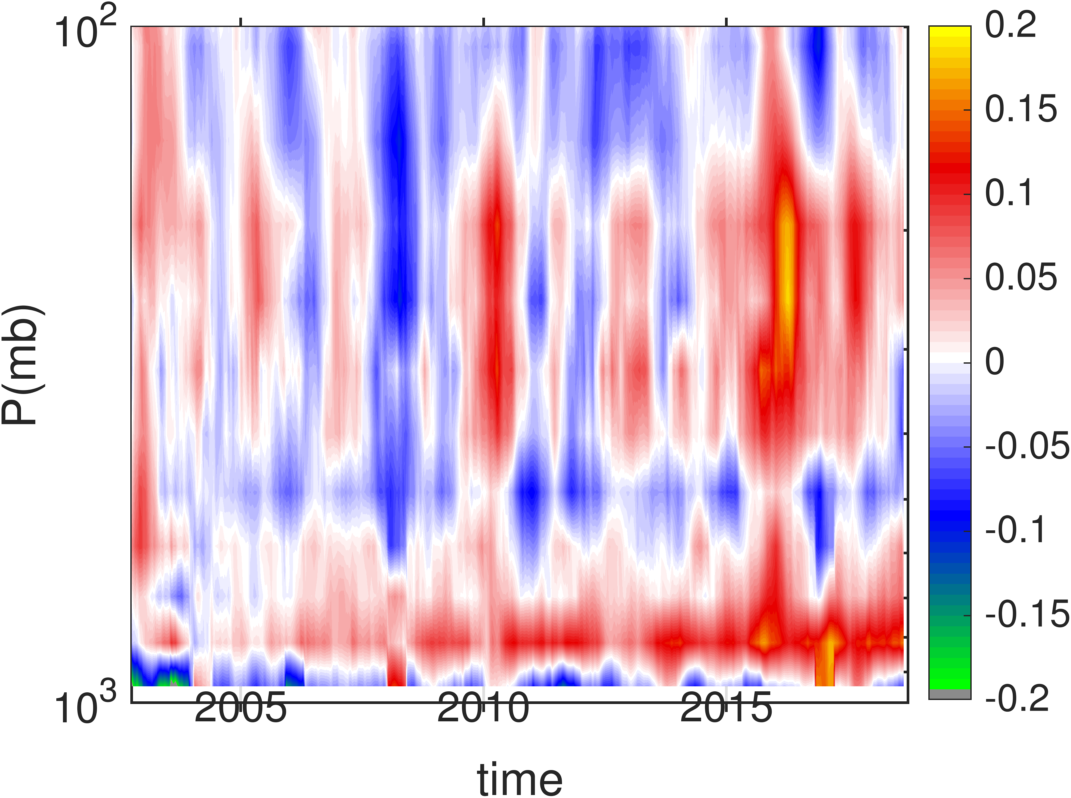
\includegraphics[width=\linewidth]{Figs/ClearAnom/umbc_clr_retr_obs_wv_anom_200209_201808.png}
\end{center}
\end{block}
\end{column}

\begin{column}{0.45\columnwidth}
\begin{block}{\footnotesize UMBC Retr Calc}
\vspace{-0.1in}
\begin{center}
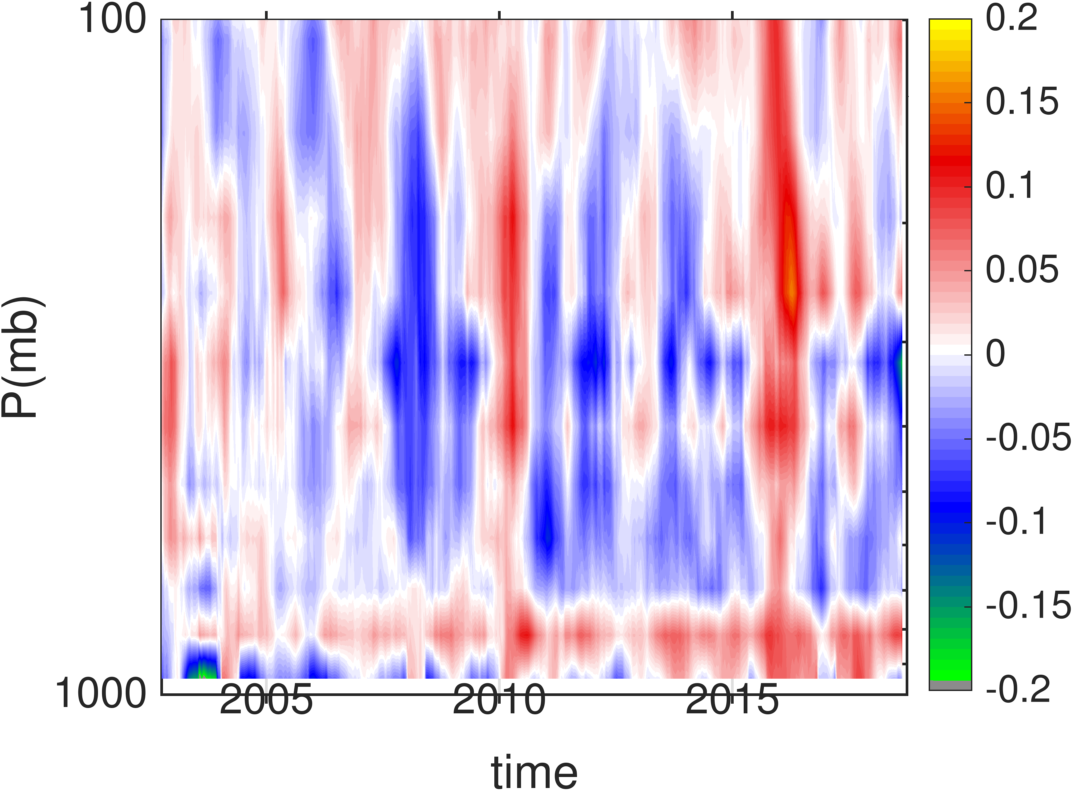
\includegraphics[width=\linewidth]{Figs/ClearAnom/umbc_clr_retr_cal_wv_anom_200209_201808.png}
\end{center}
\end{block}
\end{column}
\end{columns}

\end{frame}

%%%%%%%%%%%%%%%%%%%%%%%%%

% \begin{frame}{Tropical Clear Sky Geophysical Anomalies : \textit{frac} O3(z,t)}
% %% see /home/sergio/MATLABCODE/oem_pkg_run_sergio_AuxJacs/MakeProfs/plot_anomalies.m
% \vspace{-0.35in}

% \begin{columns}
% \begin{column}{0.45\columnwidth}
% \begin{block}{\footnotesize ERA}
% \vspace{-0.1in}
% \begin{center}
% 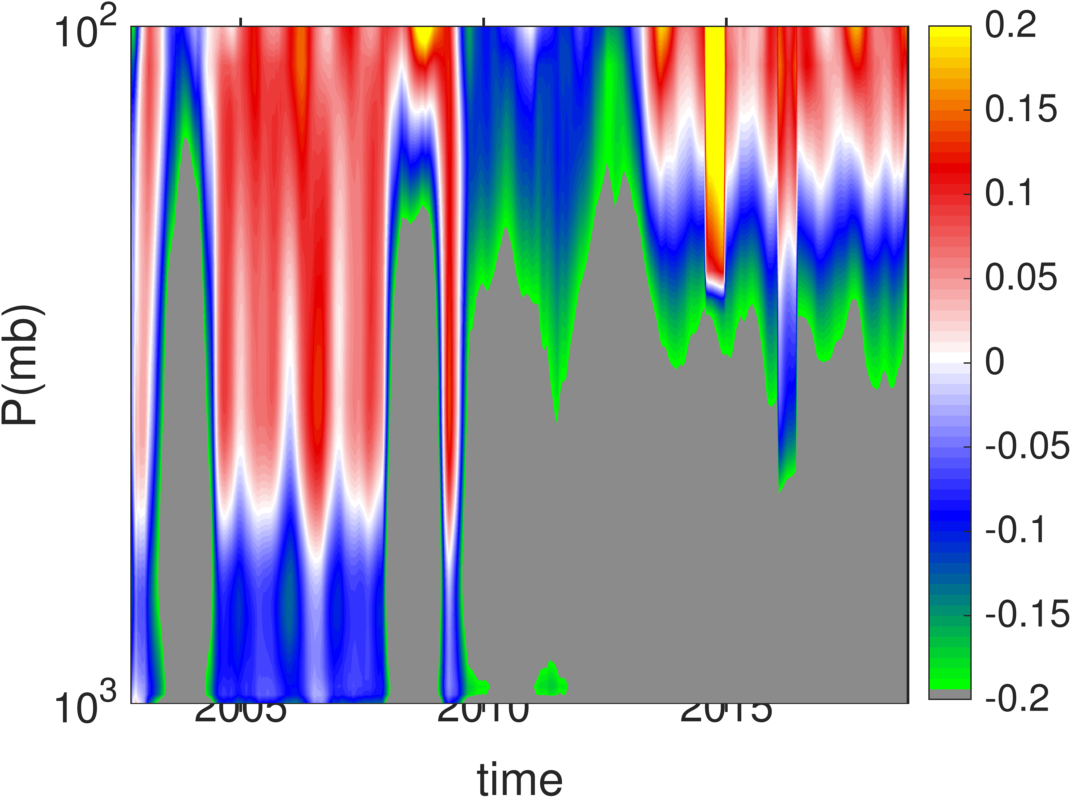
\includegraphics[width=\linewidth]{Figs/ClearAnom/era_clr_o3_anom_200209_201808.png}
% \end{center}
% \end{block}
% \end{column}

% \begin{column}{0.45\columnwidth}
% %\begin{block}{\footnotesize $frac$ O3(z,t)}
% %\vspace{-0.1in}
% %\begin{center}
% %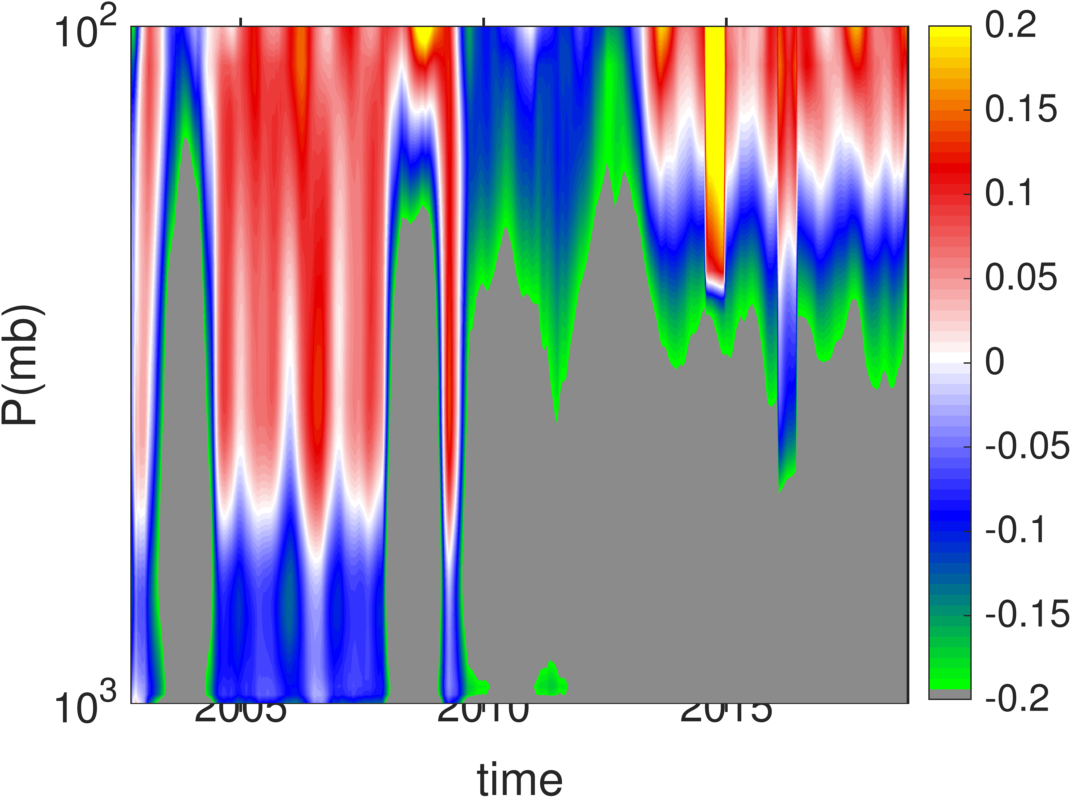
\includegraphics[width=\linewidth]{Figs/ClearAnom/era_clr_o3_anom_200209_201808.png}
% %\end{center}
% %\end{block}
% \end{column}
% \end{columns}

% \vspace{-0.25in}

% \begin{columns}
% \begin{column}{0.45\columnwidth}
% \begin{block}{\footnotesize UMBC Retr Obs}
% \vspace{-0.1in}
% \begin{center}
% 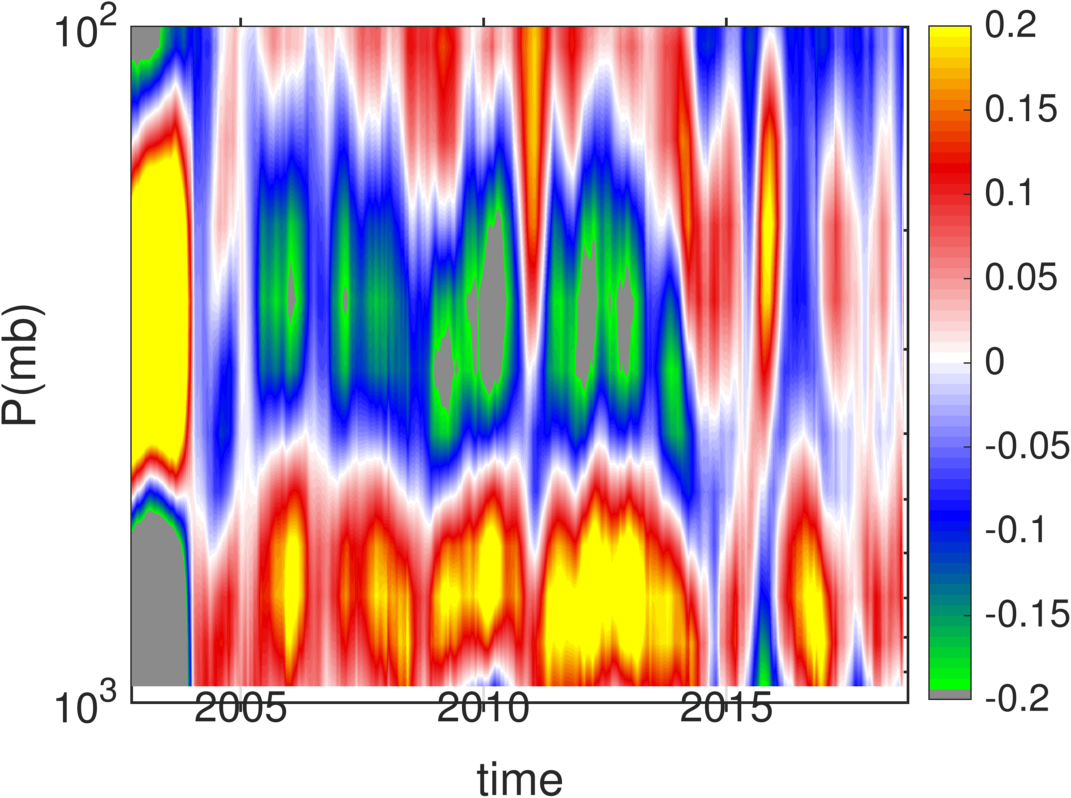
\includegraphics[width=\linewidth]{Figs/ClearAnom/umbc_clr_retr_obs_o3_anom_200209_201808.png}
% \end{center}
% \end{block}
% \end{column}

% \begin{column}{0.45\columnwidth}
% \begin{block}{\footnotesize UMBC Retr Calc}
% \vspace{-0.1in}
% \begin{center}
% 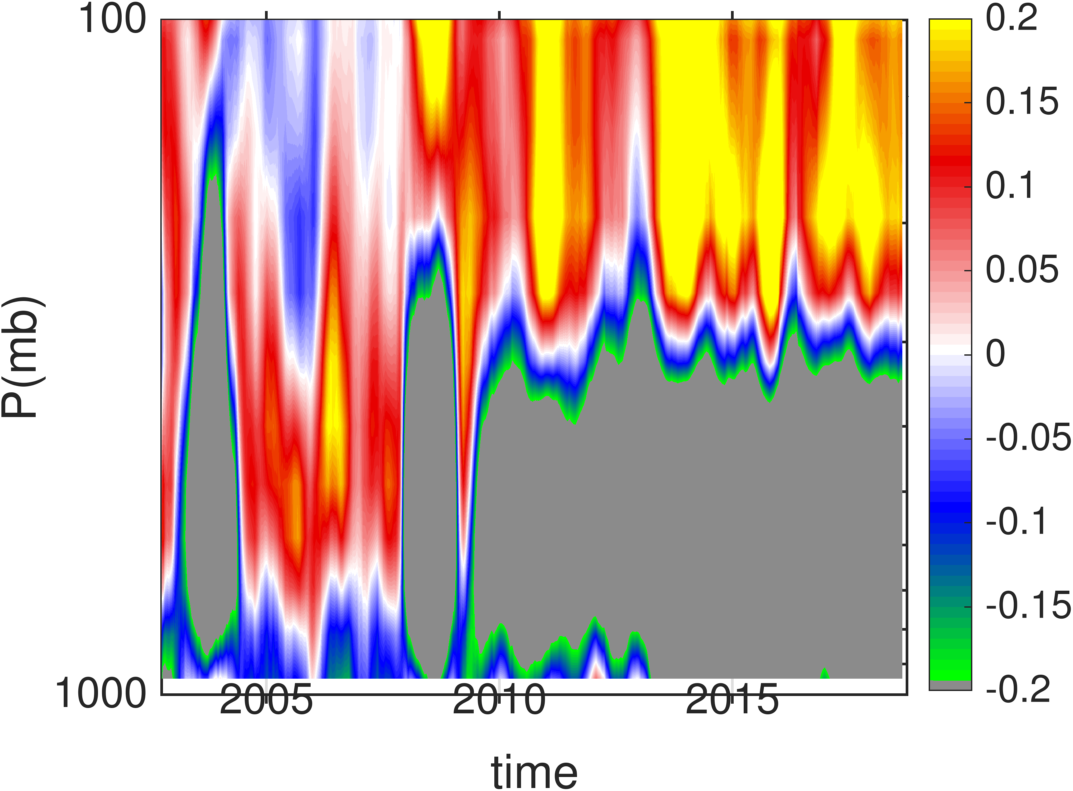
\includegraphics[width=\linewidth]{Figs/ClearAnom/umbc_clr_retr_cal_o3_anom_200209_201808.png}
% \end{center}
% \end{block}
% \end{column}
% \end{columns}

% \end{frame}

%%%%%%%%%%%%%%%%%%%%%%%%%

\begin{frame}{UMBC Retrieved Clear Sky Geophysical Anomalies $\rightarrow$ Decadal Geophysical Rates : T(z,lat)}
%% see /home/sergio/MATLABCODE/oem_pkg_run_sergio_AuxJacs/MakeProfs/plot_anomalies.m
\vspace{-0.35in}

\begin{columns}
\begin{column}{0.45\columnwidth}
\begin{block}{\footnotesize ERA}
\vspace{-0.1in}
\begin{center}
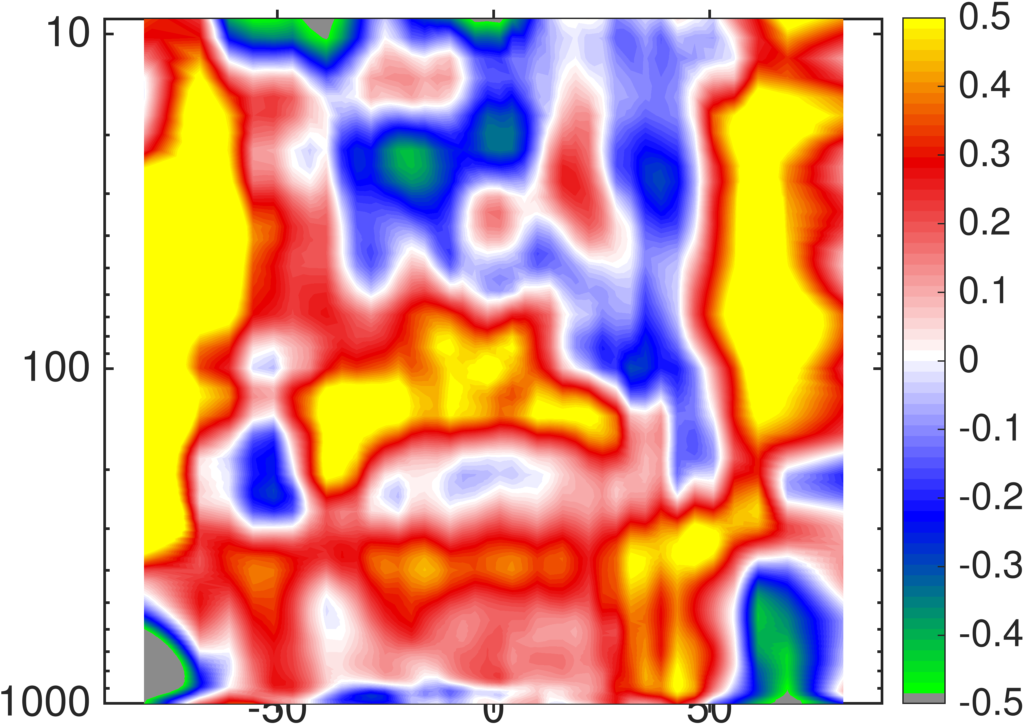
\includegraphics[width=0.95\linewidth]{Figs/ClearAnom/rawERAtzrates.png}
\end{center}
\end{block}
\end{column}

\begin{column}{0.45\columnwidth}
  \begin{block}
    
Remember: Clear sampling is extremely non-uniform spatially so expect strange structures.
\end{block}
\end{column}
\end{columns}

\vspace{-0.25in}

\begin{columns}
\begin{column}{0.45\columnwidth}
\begin{block}{\footnotesize UMBC Retr Obs}
\vspace{-0.1in}
\begin{center}
%% oops got this backwards
%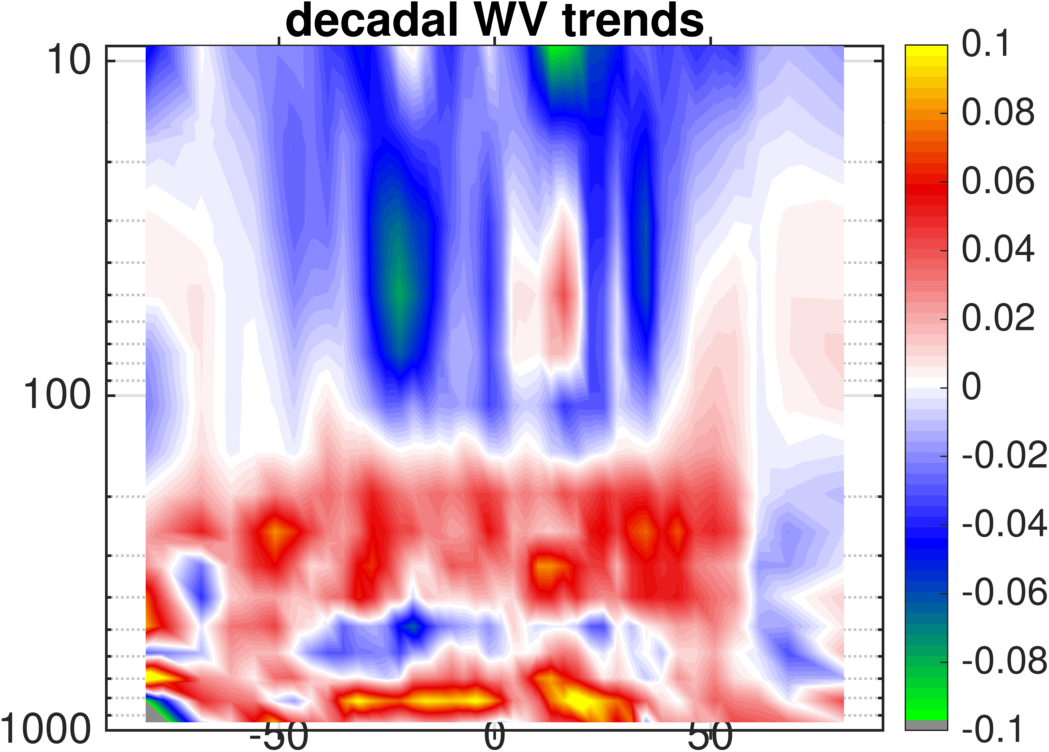
\includegraphics[width=0.95\linewidth]{Figs/ClearAnom/umbc_clr_retr_obs_ptemp_rate_200209_201808.png}
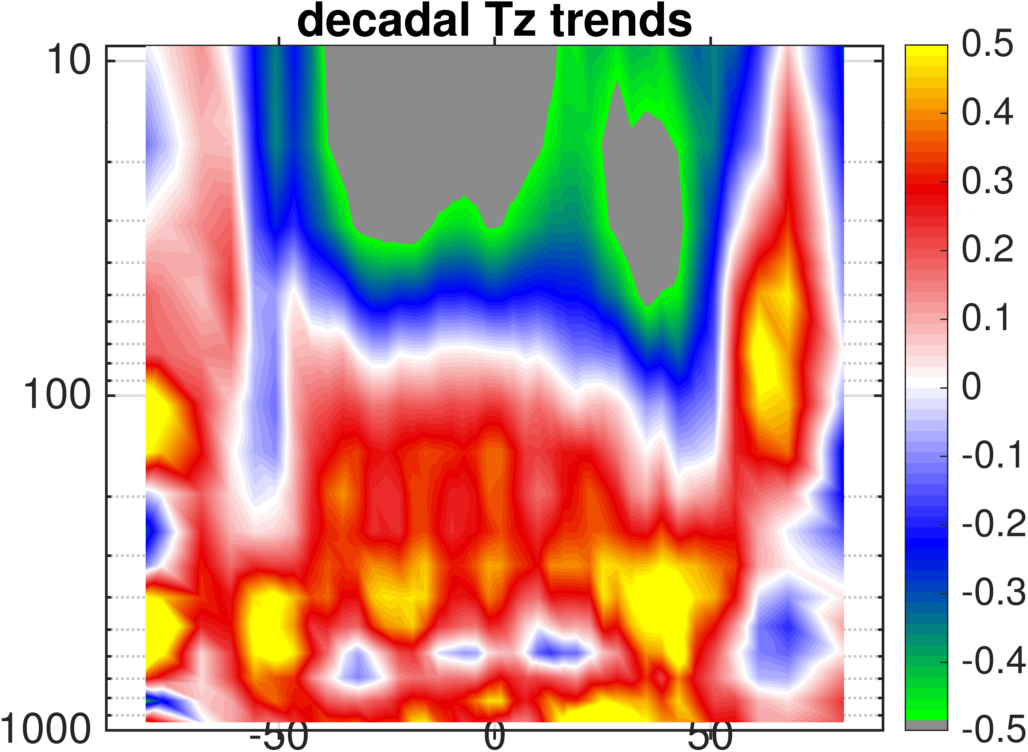
\includegraphics[width=0.95\linewidth]{Figs/ClearAnom/umbc_clr_retr_obs_wv_rate_200209_201808.png}
\end{center}
\end{block}
\end{column}

\begin{column}{0.45\columnwidth}
\begin{block}{\footnotesize UMBC Retr Calc}
\vspace{-0.1in}
\begin{center}
%% oops got this backwards
%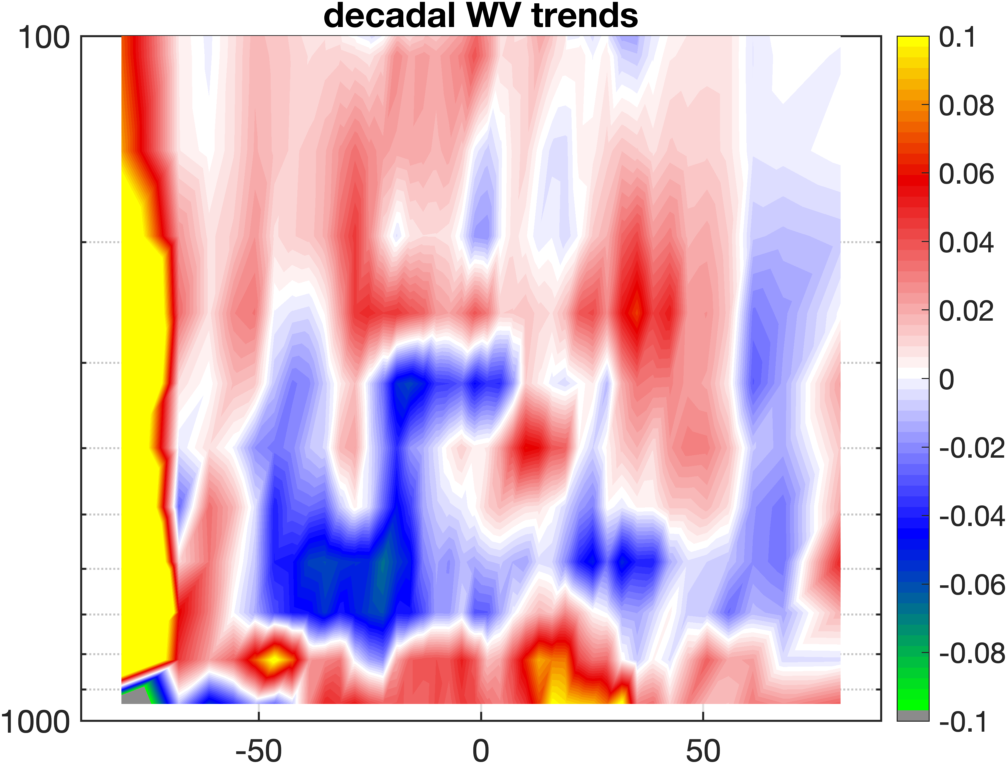
\includegraphics[width=0.95\linewidth]{Figs/ClearAnom/umbc_clr_retr_cal_ptemp_rate_200209_201808.png}
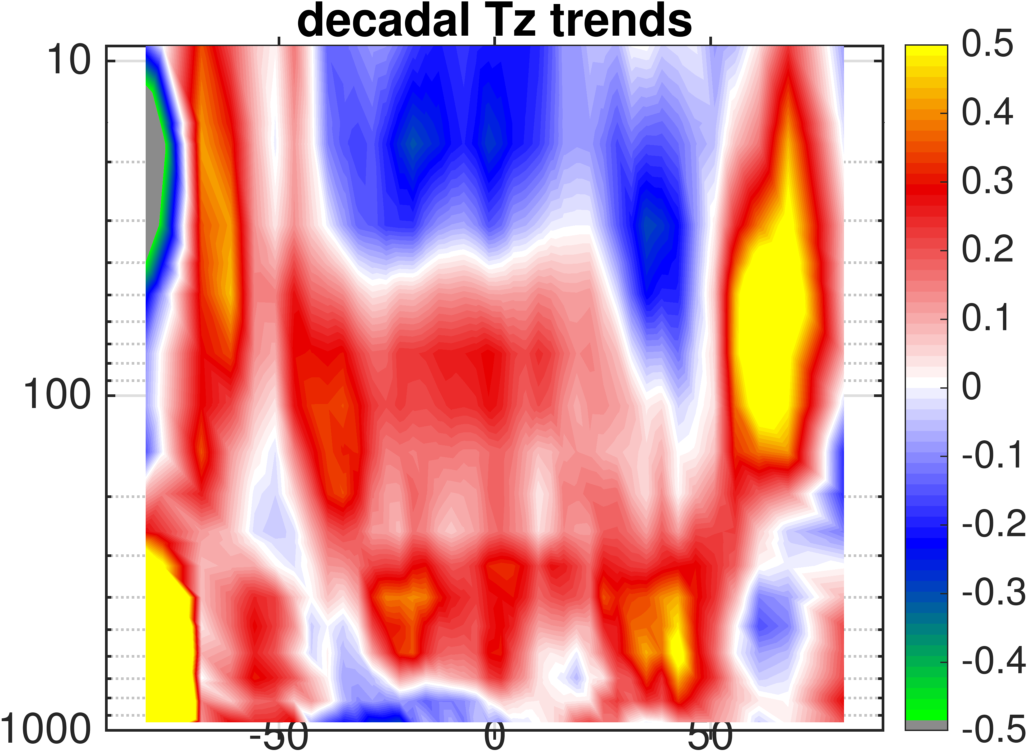
\includegraphics[width=0.95\linewidth]{Figs/ClearAnom/umbc_clr_retr_cal_wv_rate_200209_201808.png}
\end{center}
\end{block}
\end{column}
\end{columns}

\end{frame}

%%%%%%%%%%%%%%%%%%%%%%%%%

\begin{frame}{UMBC Retrieved Clear Sky Geophysical Anomalies $\rightarrow$ Decadal Geophysical Rates : WV(z,lat)}
%% see /home/sergio/MATLABCODE/oem_pkg_run_sergio_AuxJacs/MakeProfs/plot_anomalies.m
\vspace{-0.35in}

\begin{columns}
\begin{column}{0.45\columnwidth}
\begin{block}{\footnotesize ERA}
\vspace{-0.1in}
\begin{center}
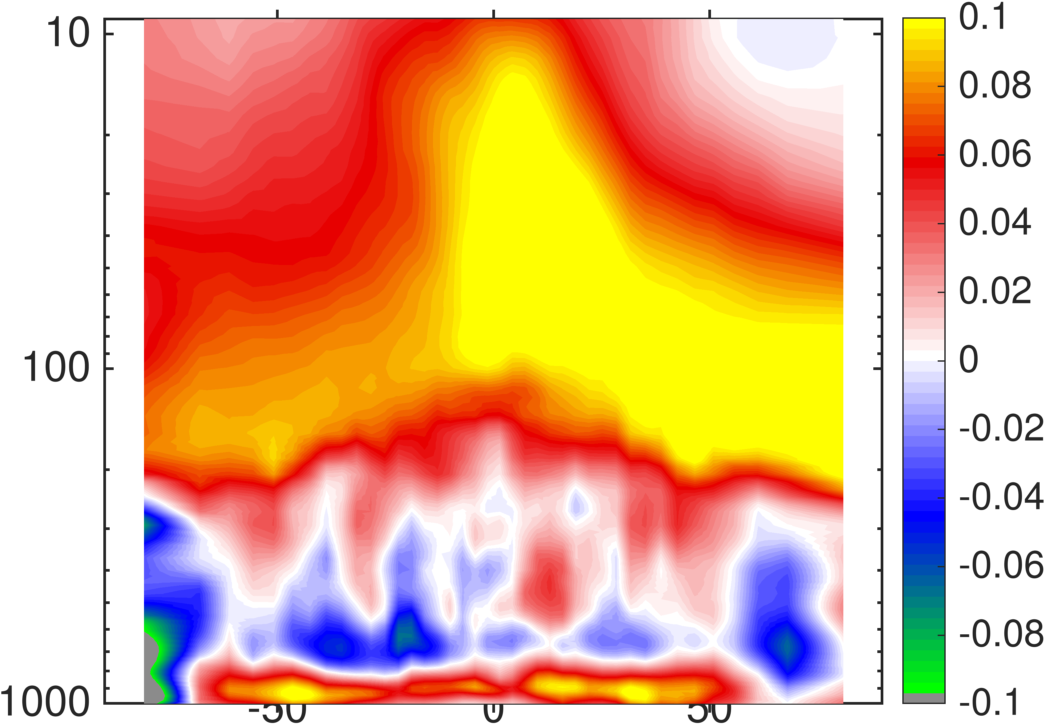
\includegraphics[width=0.95\linewidth]{Figs/ClearAnom/rawERAwvrates.png}
\end{center}
\end{block}
\end{column}

\begin{column}{0.45\columnwidth}
%\begin{block}{\footnotesize $frac$ O3(z,t)}
%\vspace{-0.1in}
%\begin{center}
%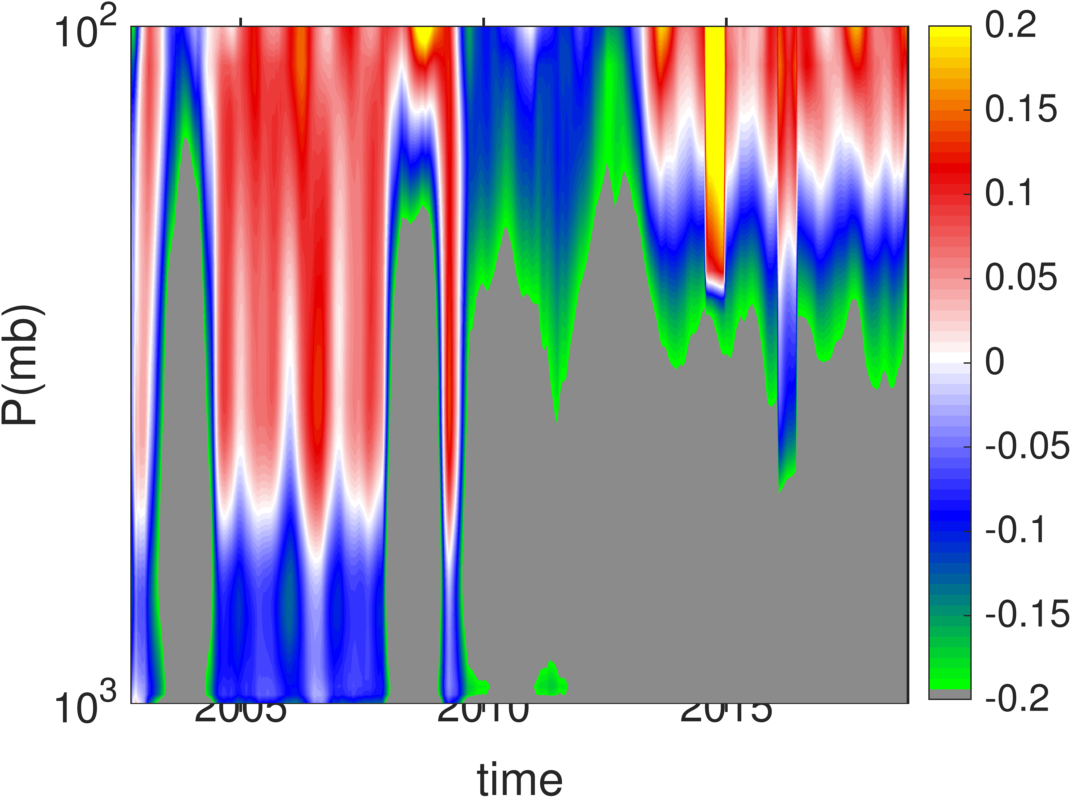
\includegraphics[width=0.95\linewidth]{Figs/ClearAnom/era_clr_o3_anom_200209_201808.png}
%\end{center}
%\end{block}
\end{column}
\end{columns}

\vspace{-0.25in}

\begin{columns}
\begin{column}{0.45\columnwidth}
\begin{block}{\footnotesize UMBC Retr Obs}
\vspace{-0.1in}
\begin{center}
%% oops got this backwards
%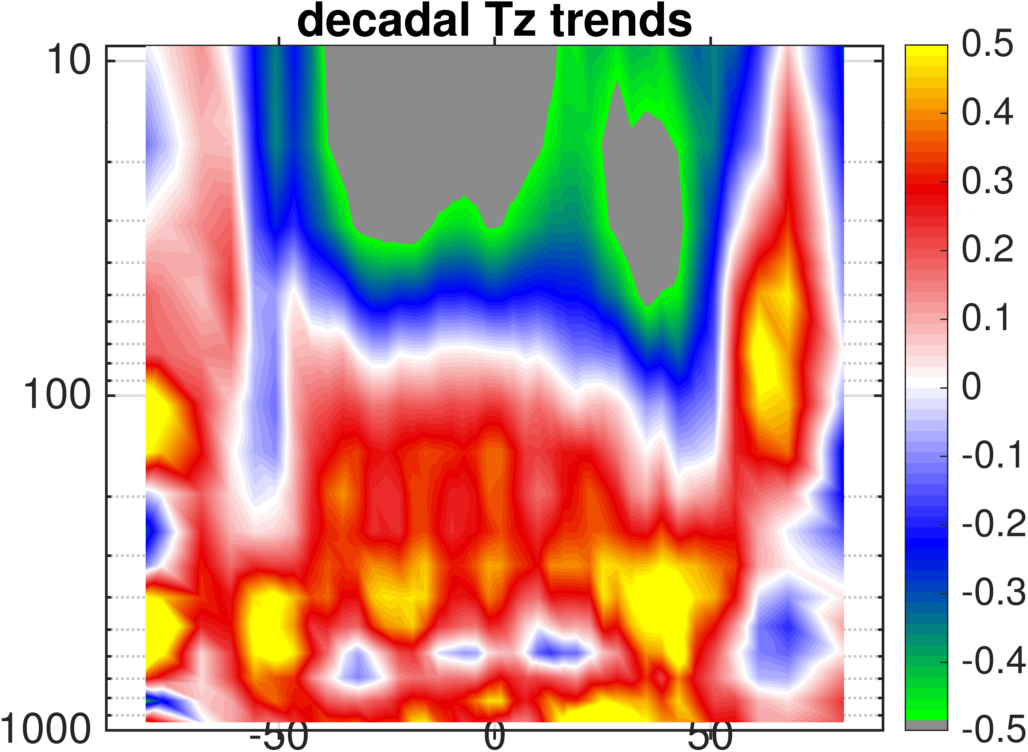
\includegraphics[width=0.95\linewidth]{Figs/ClearAnom/umbc_clr_retr_obs_wv_rate_200209_201808.png}
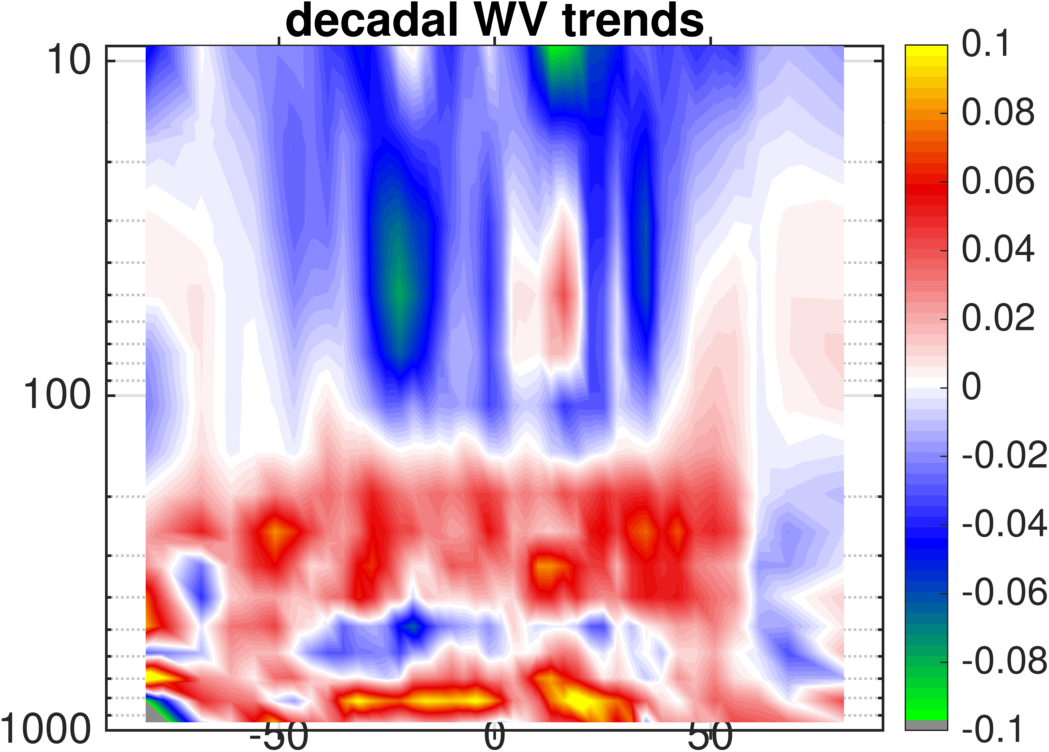
\includegraphics[width=0.95\linewidth]{Figs/ClearAnom/umbc_clr_retr_obs_ptemp_rate_200209_201808.png}
\end{center}
\end{block}
\end{column}

\begin{column}{0.45\columnwidth}
\begin{block}{\footnotesize UMBC Retr Calc}
\vspace{-0.1in}
\begin{center}
%% oops got this backwards
%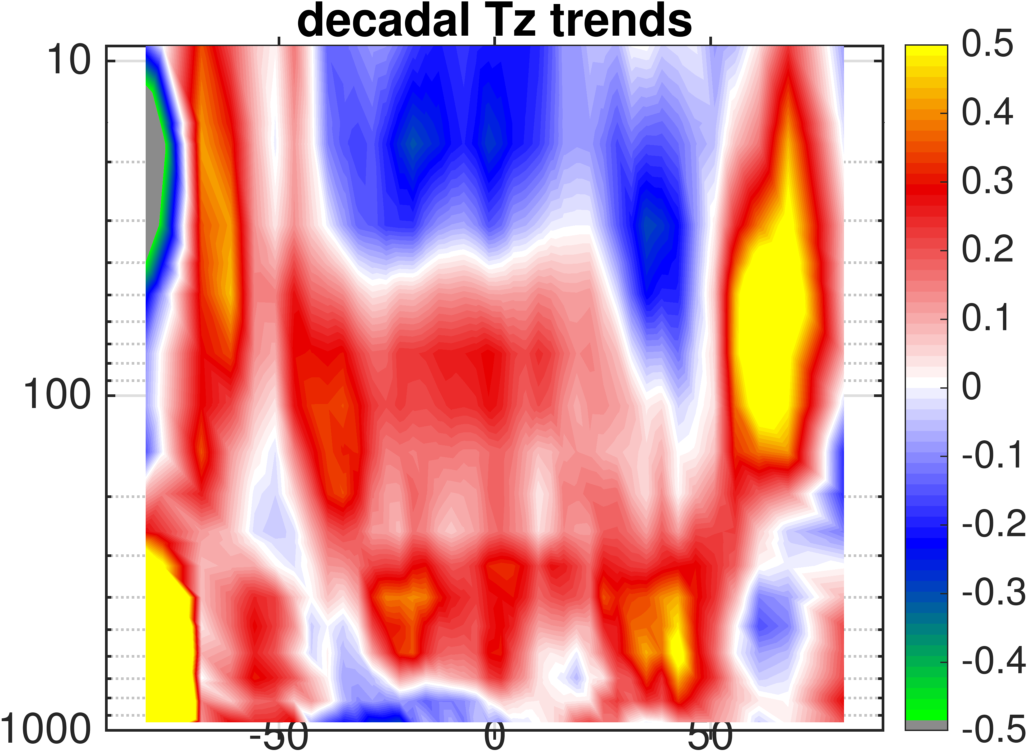
\includegraphics[width=0.95\linewidth]{Figs/ClearAnom/umbc_clr_retr_cal_wv_rate_200209_201808.png}
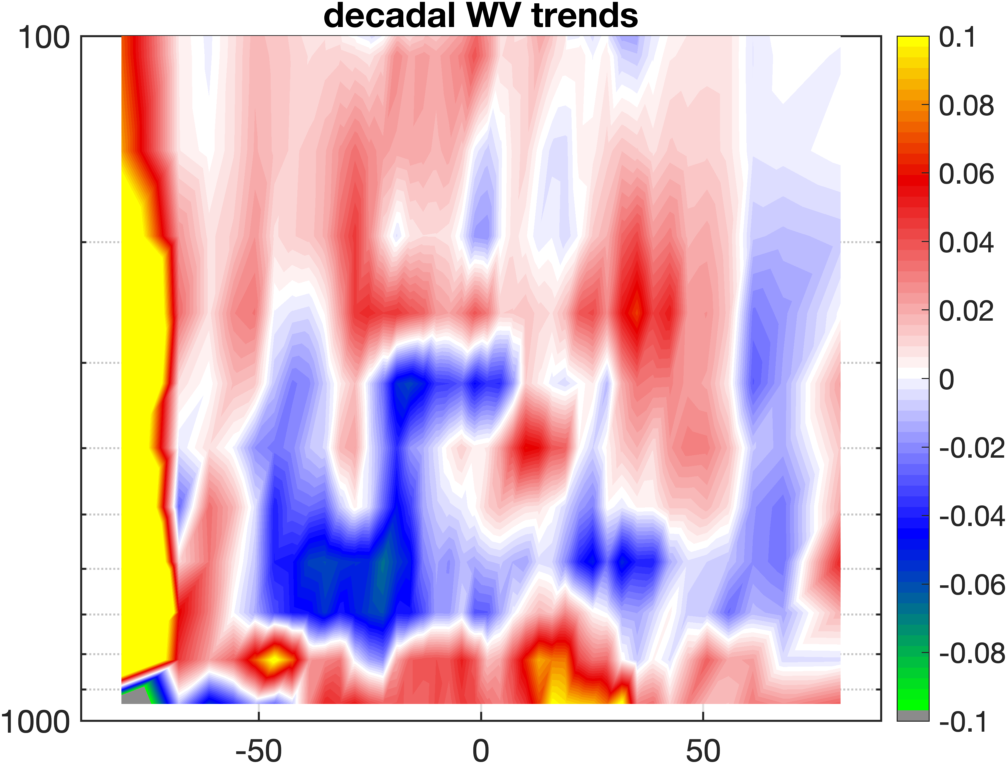
\includegraphics[width=0.95\linewidth]{Figs/ClearAnom/umbc_clr_retr_cal_ptemp_rate_200209_201808.png}
\end{center}
\end{block}
\end{column}
\end{columns}

\end{frame}

%%%%%%%%%%%%%%%%%%%%%%%%%

% \begin{frame}{UMBC Retrieved Clear Sky Geophysical Anomalies $\rightarrow$ Decadal Geophysical Rates : O3(z,lat)}
% %% see /home/sergio/MATLABCODE/oem_pkg_run_sergio_AuxJacs/MakeProfs/plot_anomalies.m
% \vspace{-0.35in}

% \begin{columns}
% \begin{column}{0.45\columnwidth}
% \begin{block}{\footnotesize ERA}
% \vspace{-0.1in}
% \begin{center}
% 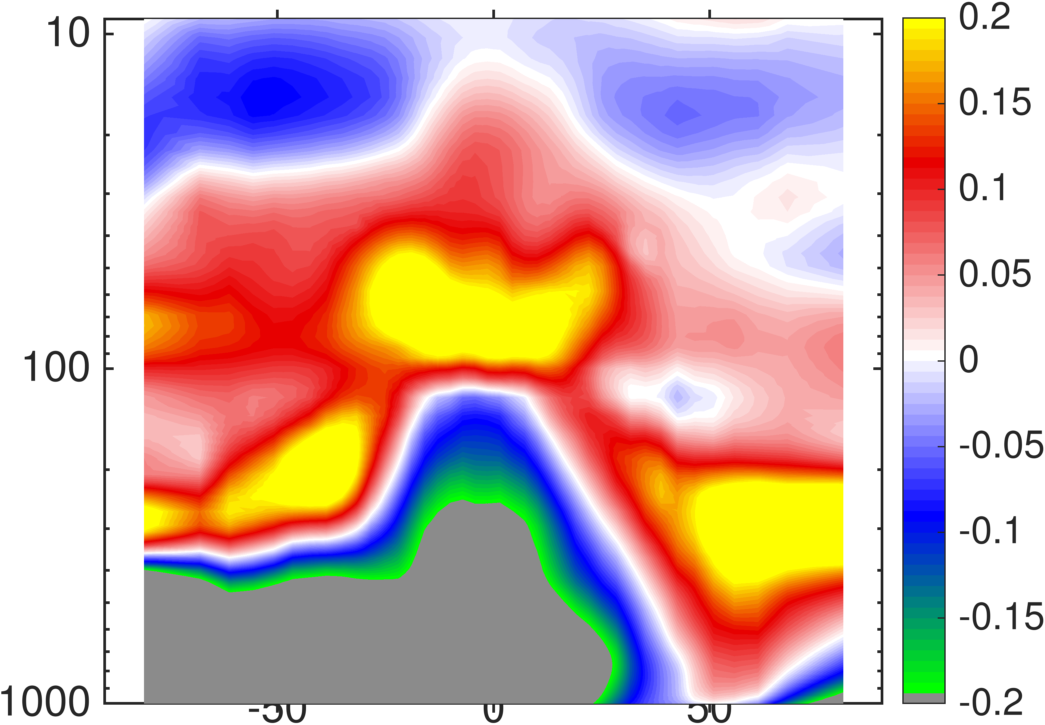
\includegraphics[width=\linewidth]{Figs/ClearAnom/rawERAo3rates.png}
% \end{center}
% \end{block}
% \end{column}

% \begin{column}{0.45\columnwidth}
% %\begin{block}{\footnotesize $frac$ O3(z,t)}
% %\vspace{-0.1in}
% %\begin{center}
% %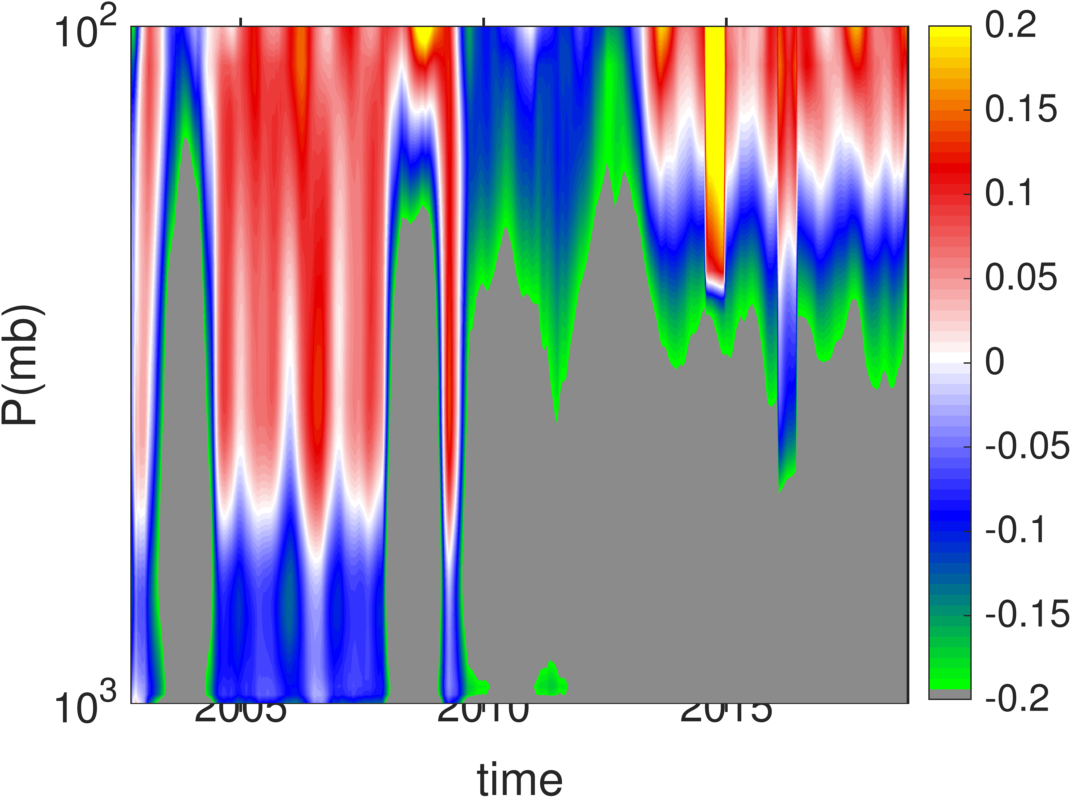
\includegraphics[width=\linewidth]{Figs/ClearAnom/era_clr_o3_anom_200209_201808.png}
% %\end{center}
% %\end{block}
% \end{column}
% \end{columns}

% \vspace{-0.25in}

% \begin{columns}
% \begin{column}{0.45\columnwidth}
% \begin{block}{\footnotesize UMBC Retr Obs}
% \vspace{-0.1in}
% \begin{center}
% 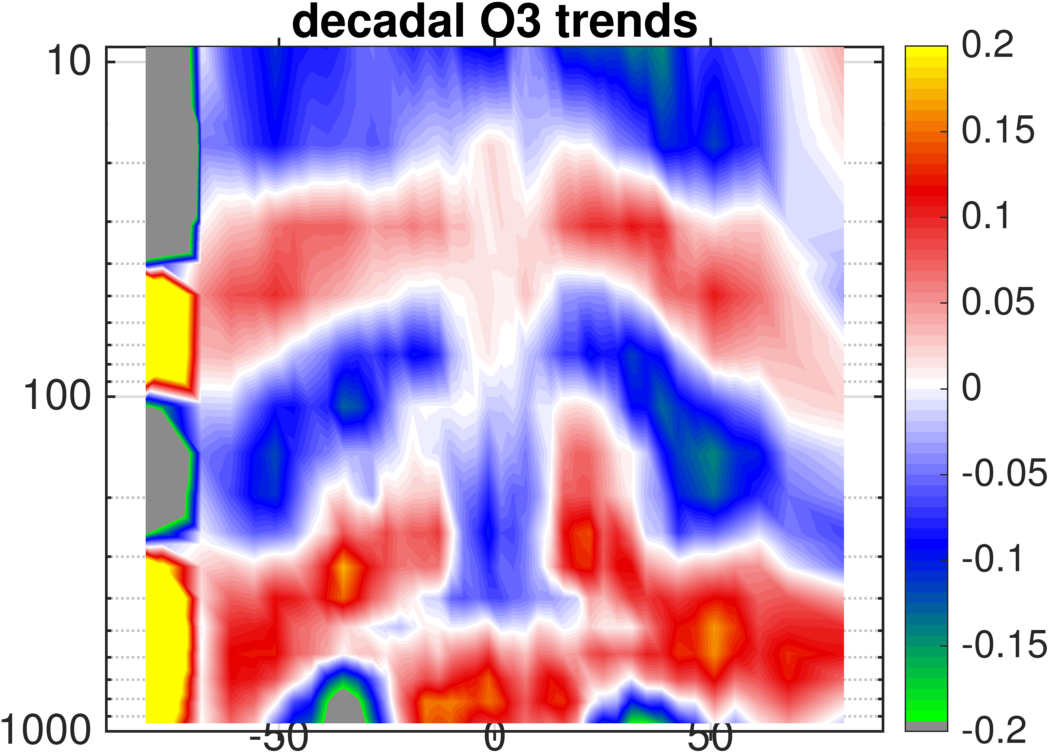
\includegraphics[width=\linewidth]{Figs/ClearAnom/umbc_clr_retr_obs_o3_rate_200209_201808.png}
% \end{center}
% \end{block}
% \end{column}

% \begin{column}{0.45\columnwidth}
% \begin{block}{\footnotesize UMBC Retr Calc}
% \vspace{-0.1in}
% \begin{center}
% 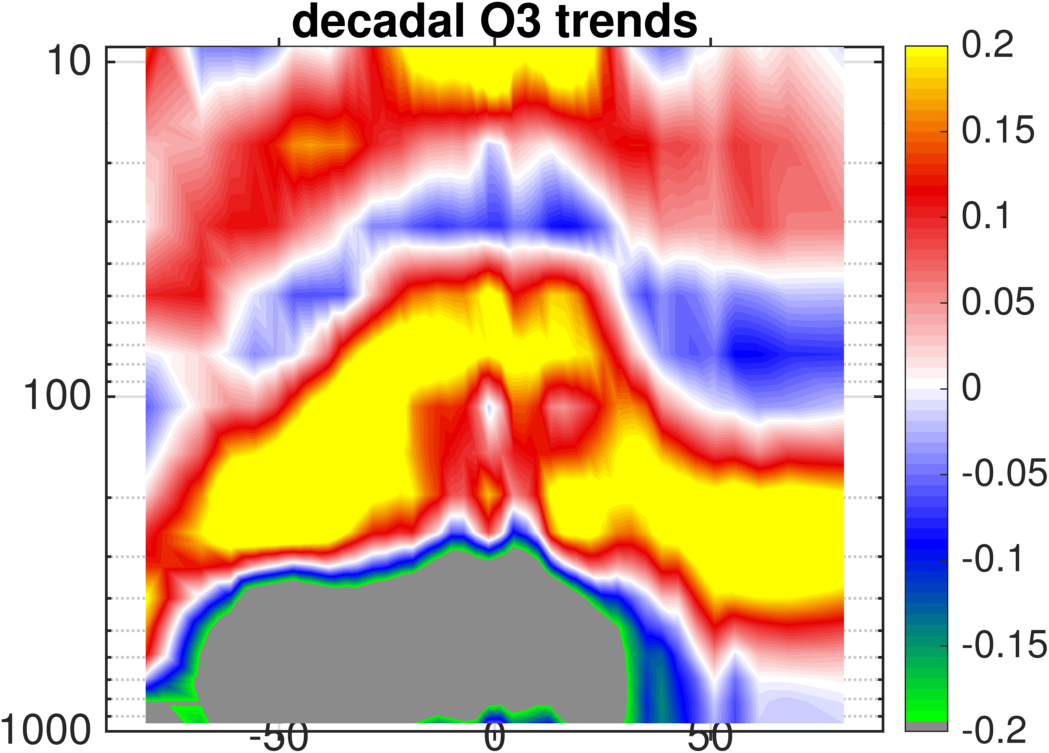
\includegraphics[width=\linewidth]{Figs/ClearAnom/umbc_clr_retr_cal_o3_rate_200209_201808.png}
% \end{center}
% \end{block}
% \end{column}
% \end{columns}

% \end{frame}
%%%%%%%%%%%%%%%%%%%%%%%%%
%%%%%%%%%%%%%%%%%%%%%%%%%%%%%%%%%%%%%%%%%%%%%%%%%%%%%%%%%%%%%%%%%%%%%%%%%%%
% ---------------------------------------------------------------------
\section{AllSky Results}

\begin{frame}
  \frametitle{AllSky Retrievals}
  \begin{itemize}
    \item \textcolor{red}{Interested in a less specialized sampling, so will now look at allsky rates}
    \item Larrabee's talk gives details (data from 2002/09 to 2018/08)
      \begin{itemize}
        \item binned into 40 equal area latitude bins (thinner in equator/thicker at polar regions)
        \item \textcolor{red}{AIRS observations randomly sampled from these bins}
        \item 16 years of data divided into 16 day averages $\rightarrow$ 365 timesteps
        \item BT anomalies and average ERA profiles for all 365 timesteps
      \end{itemize}
    \item kCARTA analytic jacobians for surface temperature, T(z), WV(z),O3(z) using TwoSlab Clouds
          and also for trace gases(CO2,N2O,CH4,CFC11,CFC12)
    \item SARTA for cloud jacs (kCARTA and SARTA slightly differ in cloud vertical placement)
    \item Using these jacobians, we retrieved T(t,z),WV(t,z),O3(t,z),[CO2(t),N2O(t),CH4(t),CFC11(t),CFC12(t),surftemp(t)]
          [cld amount/cld eff size/ cld top for liquid/ice clouds] at each of the 40 latbins $\times $ 365 timesteps
  \end{itemize}
\end{frame}

%%%%%%%%%%%%%%%%%%%%%%%%%

\section{AllSky OCEAN}
\subsection{AllSky spectra over ocean $\rightarrow$ geophysical rates}

\begin{frame}{Trace gas + stemp rates from spectral rates}
\vspace{-0.3in}

\begin{columns}
\begin{column}{0.55\columnwidth}
\begin{block}{\footnotesize Stemp Rates}
\vspace{-0.1in}
\begin{center}
\includegraphics[width=\linewidth]{Figs/CloudAnom/Desc_ocean/stemp_lat_rates_from_obs_specral_rates.pdf}
\end{center}
\footnotesize
\begin{itemize}
\item   Ocean only
\item -25 deg. lat bump is a cloud problem
  \item gridded anomalies should remove this problem
\end{itemize}
\end{block}
\end{column}

\begin{column}{0.55\columnwidth}
%\begin{block}{\footnotesize Cloud param rates}
\begin{block}{\footnotesize Trace gas rates}
\vspace{-0.1in}
\begin{center}
%\includegraphics[width=\linewidth]{Figs/CloudAnom/Desc_ocean/cloudparam_lat_rates_from_obs_specral_rates.pdf}
\includegraphics[width=\linewidth]{Figs/CloudAnom/Desc_ocean/tracegas_lat_rates_from_obs_specral_rates.pdf}
\end{center}
\footnotesize
Preliminary work
\end{block}
\end{column}
\end{columns}
\end{frame}

%%%%%%%%%%

%figure(1);  aslprint_mat('/home/sergio/PAPERS/AIRS/airs_stm_sep19/allsky/Figs/CloudAnom/Desc_ocean/wv_lat_p_rates_from_obs_specral_rates',1,1,latx,playsRET,temp_ret*10);
%figure(2);  aslprint_mat('/home/sergio/PAPERS/AIRS/airs_stm_sep19/allsky/Figs/CloudAnom/Desc_ocean/tz_lat_p_rates_from_obs_specral_rates',2,1,latx,playsRET,temp_ret*10);
%figure(3);  aslprint_mat('/home/sergio/PAPERS/AIRS/airs_stm_sep19/allsky/Figs/CloudAnom/Desc_ocean/o3_lat_p_rates_from_obs_specral_rates',3,1,latx,playsRET,temp_ret*10);
%figure(7);  aslprint('/home/sergio/PAPERS/AIRS/airs_stm_sep19/allsky/Figs/CloudAnom/Desc_ocean/tracegas_lat_rates_from_obs_specral_rates.pdf');
%figure(9);  aslprint('/home/sergio/PAPERS/AIRS/airs_stm_sep19/allsky/Figs/CloudAnom/Desc_ocean/stemp_lat_rates_from_obs_specral_rates.pdf');
%figure(10); aslprint('/home/sergio/PAPERS/AIRS/airs_stm_sep19/allsky/Figs/CloudAnom/Desc_ocean/cloudparam_lat_rates_from_obs_specral_rates.pdf')

%% see /home/sergio/MATLABCODE/oem_pkg_run/AIRS_new_random_scan_August2019/Plotutils/plot_all_latbins_fewlays.m
%% see /home/sergio/MATLABCODE/oem_pkg_run_sergio_AuxJacs/MakeProfs/plot_anomalies.m
\begin{frame}{Comparing ERA versus UMBC AllSky Geophysical Rates : dT(z,lat)/dt}
\vspace{-0.35in}

\begin{columns}
\begin{column}{0.55\columnwidth}
\begin{block}{\footnotesize ERA}
\vspace{-0.1in}
\begin{center}
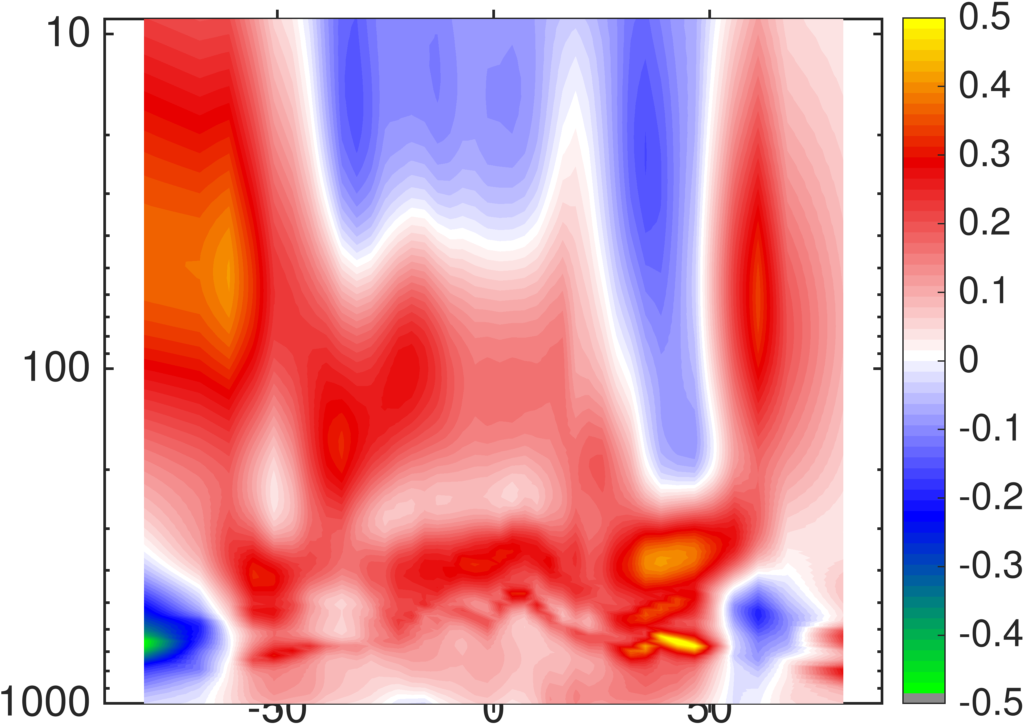
\includegraphics[width=0.925\linewidth]{Figs/CloudAnom/Desc_ocean/ak_x_ERAtzrates.png}
\end{center}
\end{block}
\end{column}

\begin{column}{0.55\columnwidth}
%\begin{block}{\footnotesize Cloud param rates}
\begin{block}{\footnotesize UMBC}
\vspace{-0.1in}
\begin{center}
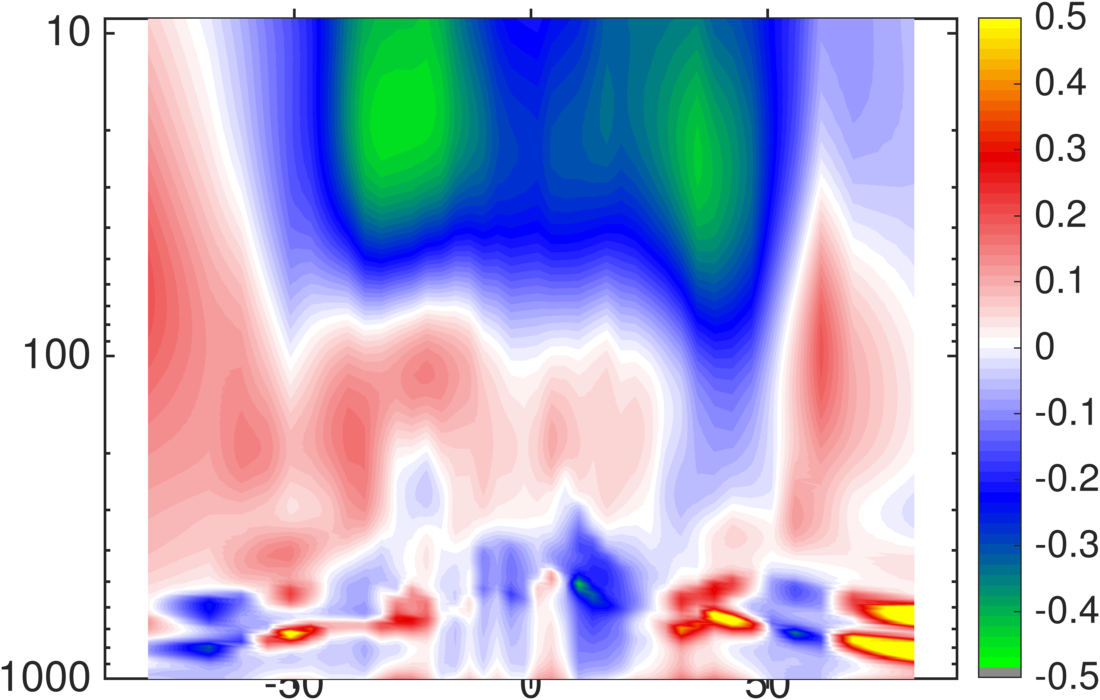
\includegraphics[width=\linewidth]{Figs/CloudAnom/Desc_ocean/tz_lat_p_rates_from_obs_specral_rates.png}
\end{center}
\end{block}
\end{column}
\end{columns}

-  Again, these are zonal all-sky retrievals that combine greatly variable longitudal trends, mostly due to cloud variability during ENSO periods.

- Switching to gridded retrievals should help improve cloud paramater retrievals.

\end{frame}

%%%%%
\begin{frame}{Comparing ERA versus UMBC AllSky Geophysical Rates : dWV(z,lat)/dt}
\vspace{-0.35in}

\begin{columns}
\begin{column}{0.55\columnwidth}
\begin{block}{\footnotesize ERA}
\vspace{-0.1in}
\begin{center}
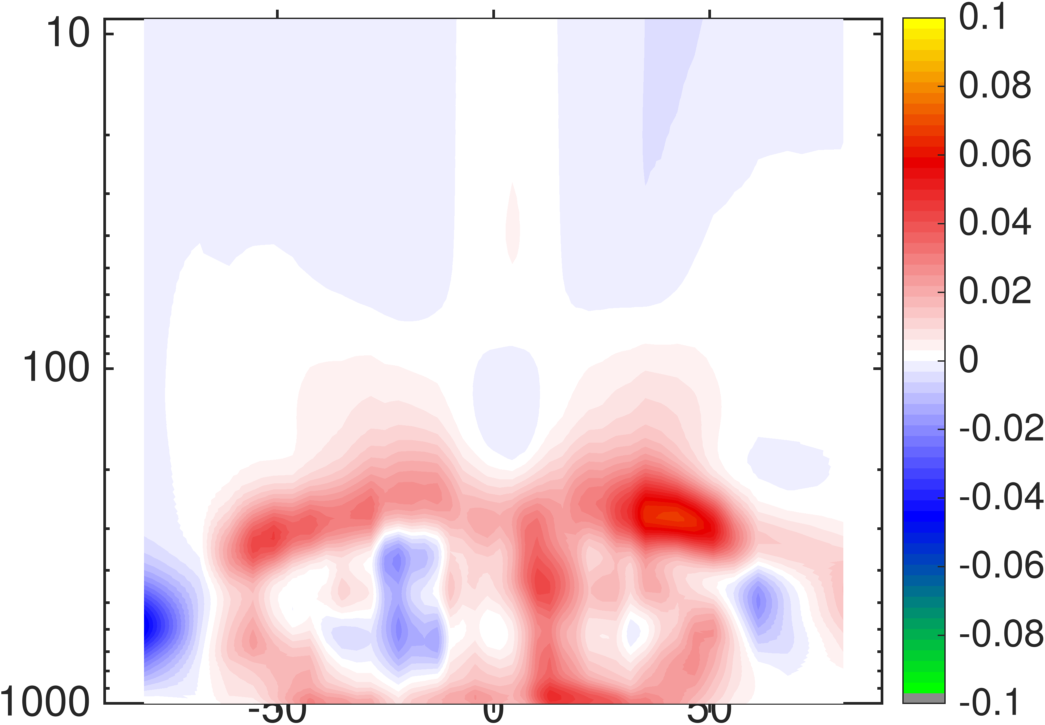
\includegraphics[width=0.925\linewidth]{Figs/CloudAnom/Desc_ocean/ak_x_ERAwvrates.png}
\end{center}
\end{block}
\end{column}

\begin{column}{0.55\columnwidth}
%\begin{block}{\footnotesize Cloud param rates}
\begin{block}{\footnotesize UMBC}
\vspace{-0.1in}
\begin{center}
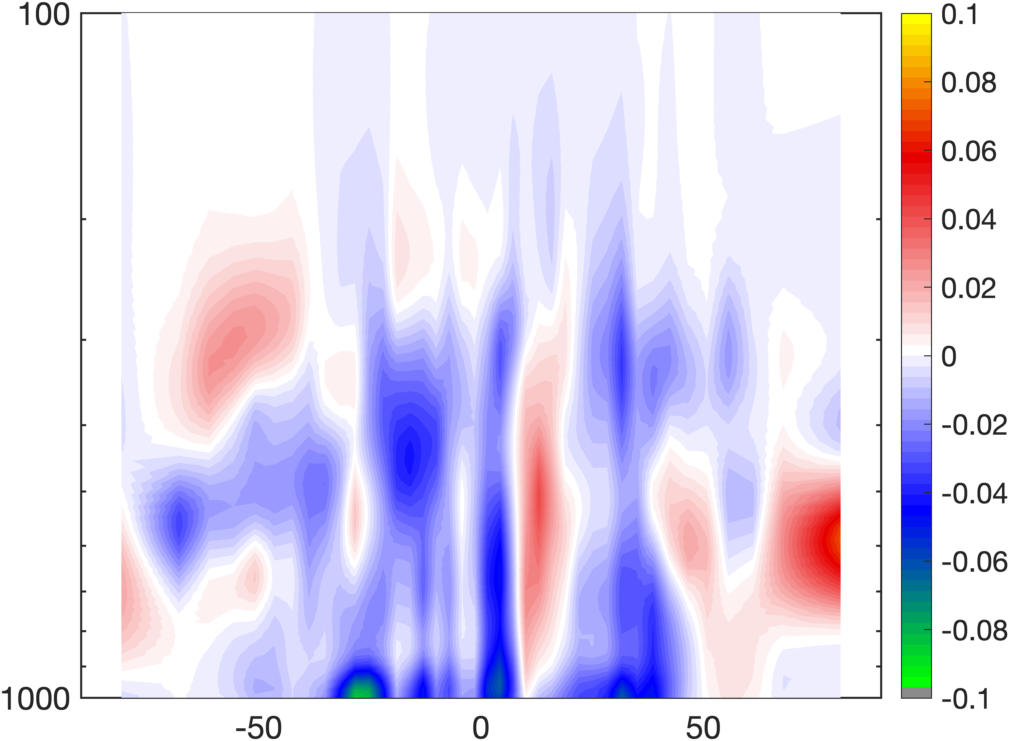
\includegraphics[width=\linewidth]{Figs/CloudAnom/Desc_ocean/wv_lat_p_rates_from_obs_specral_rates.png}
\end{center}
\end{block}
\end{column}
\end{columns}
Note: global radiance trends suggest AIRS water trends are lower than ERA.

\end{frame}

%%%%%
\begin{frame}{Comparing ERA versus UMBC AllSky Geophysical Rates : dO3(z,lat)/dt}
\vspace{-0.35in}

\begin{columns}
\begin{column}{0.55\columnwidth}
\begin{block}{\footnotesize ERA}
\vspace{-0.1in}
\begin{center}
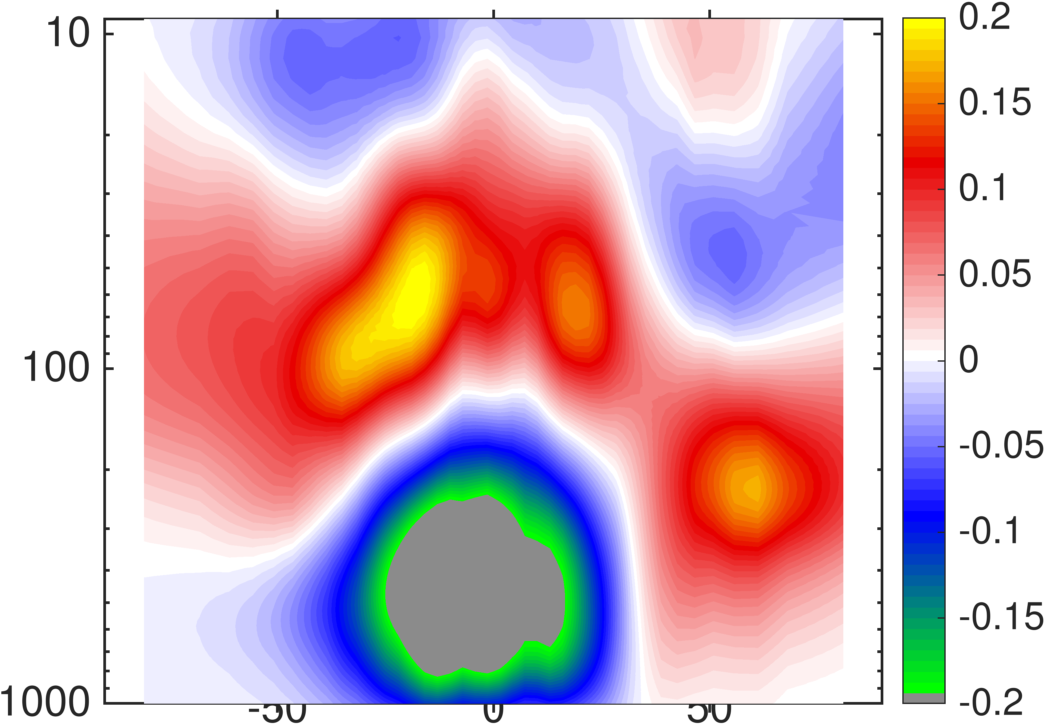
\includegraphics[width=0.925\linewidth]{Figs/CloudAnom/Desc_ocean/ak_x_ERAo3rates.png}
\end{center}
\end{block}
\end{column}

\begin{column}{0.55\columnwidth}
%\begin{block}{\footnotesize Cloud param rates}
\begin{block}{\footnotesize UMBC}
\vspace{-0.1in}
\begin{center}
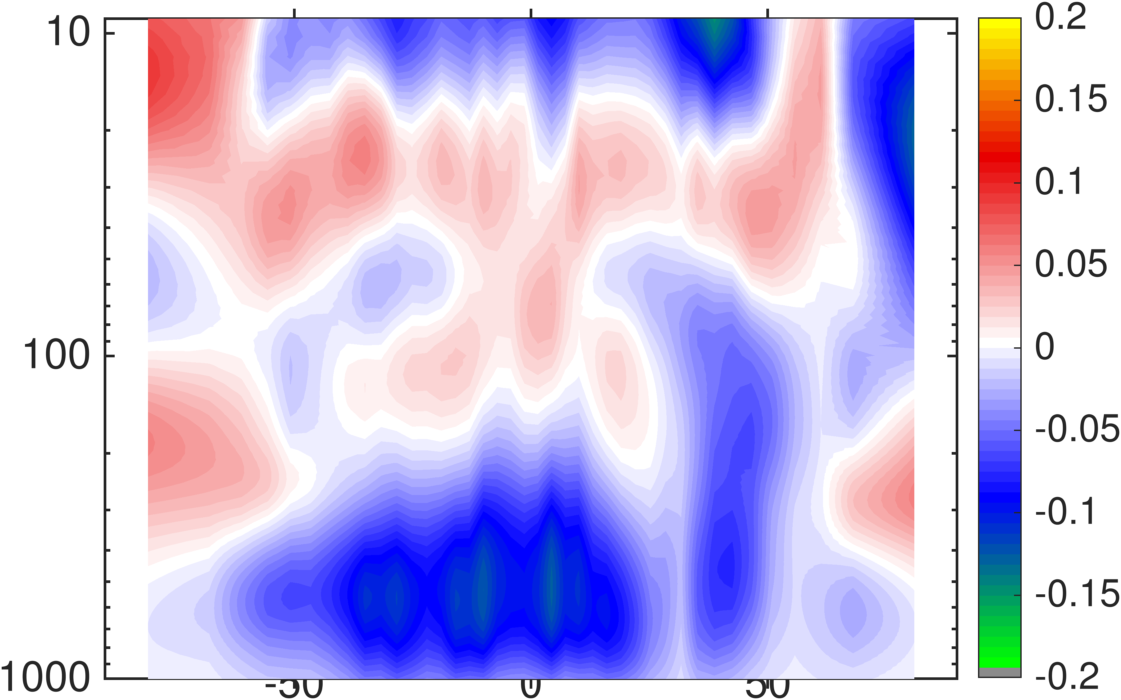
\includegraphics[width=\linewidth]{Figs/CloudAnom/Desc_ocean/o3_lat_p_rates_from_obs_specral_rates.png}
\end{center}
\end{block}
\end{column}
\end{columns}


\end{frame}

%%%%%
%%%%%

\begin{frame}{27 N AllSky Ocean Geophysical Anomalies : T(z,t)}
%% see /home/sergio/MATLABCODE/oem_pkg_run_sergio_AuxJacs/MakeProfs/plot_anomalies.m
\vspace{-0.35in}

\begin{columns}
\begin{column}{0.55\columnwidth}
\begin{block}{\footnotesize ERA}
\vspace{-0.1in}
\begin{center}
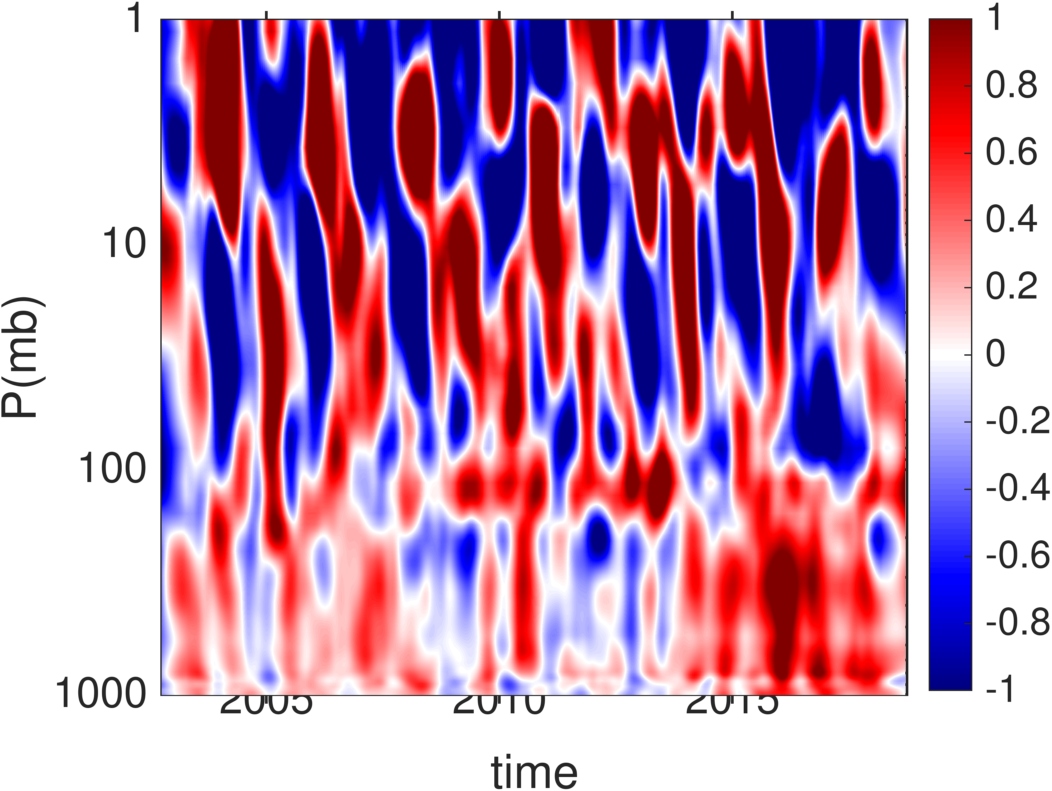
\includegraphics[width=0.9\linewidth]{Figs/CloudAnom/Desc_ocean/ntropics27_era_cld_ptemp_anom_200209_201808.png}
\end{center}
\end{block}
\end{column}

\begin{column}{0.55\columnwidth}
\begin{block}{}
  \begin{itemize}
  \item Appears our AK smoothing is too strong.
    \item Insufficient regularization low in the atmosphere.
  \end{itemize}
\end{block}
\end{column}
\end{columns}

\vspace{-0.45in}

\begin{columns}
\begin{column}{0.55\columnwidth}
\begin{block}{\footnotesize <AK> x ERA}
\vspace{-0.1in}
\begin{center}
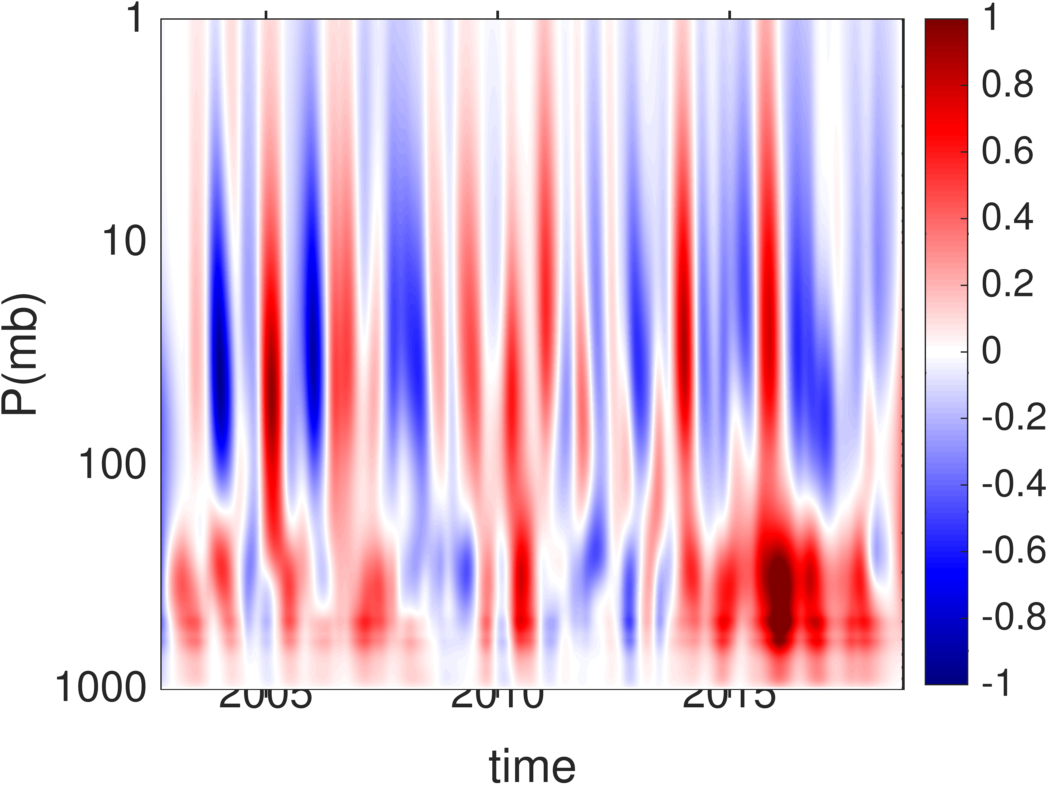
\includegraphics[width=0.95\linewidth]{Figs/CloudAnom/Desc_ocean/ak_x_ntropics27_era_cld_ptemp_anom_200209_201808.png}
\end{center}
\end{block}
\end{column}

\begin{column}{0.55\columnwidth}
%\begin{block}{\footnotesize Cloud param rates}
\begin{block}{\footnotesize UMBC}
\vspace{-0.1in}
\begin{center}
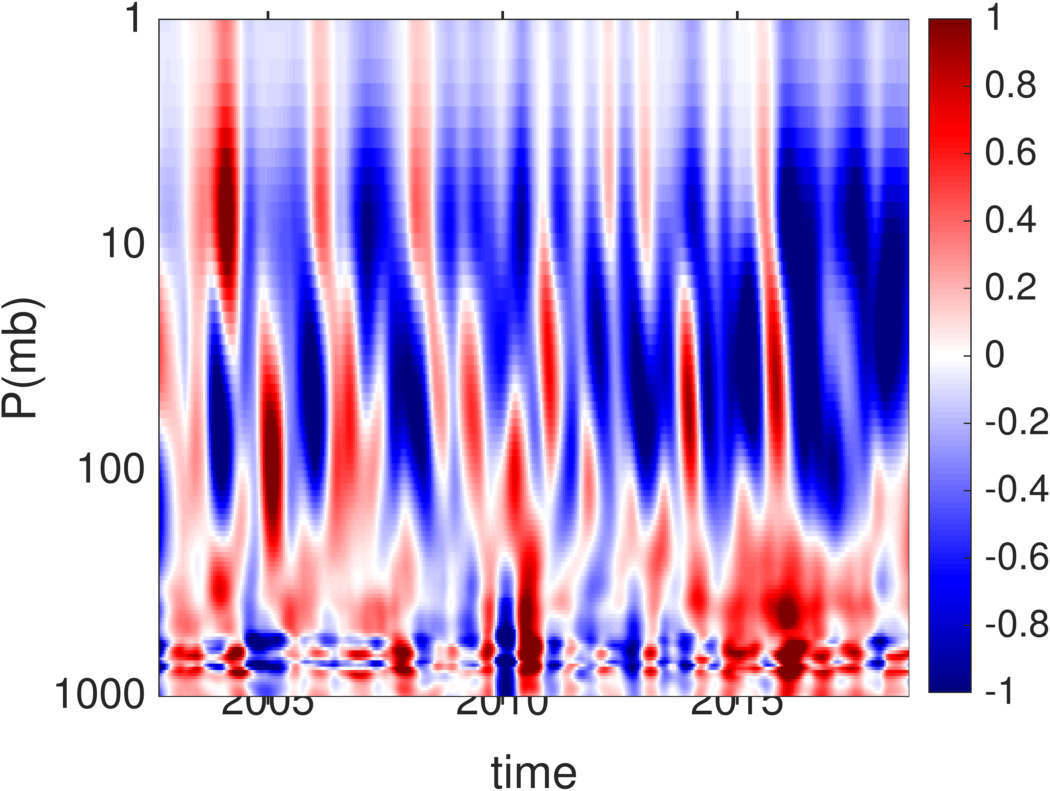
\includegraphics[width=0.95\linewidth]{Figs/CloudAnom/Desc_ocean/ntropic27N_umbc_cld_retr_obs_ptemp_anom_200209_201808.png}
\end{center}
\end{block}
\end{column}
\end{columns}

\end{frame}

\begin{frame}{27 N AllSky Ocean Geophysical Anomalies : WV(z,t)}
%% see /home/sergio/MATLABCODE/oem_pkg_run_sergio_AuxJacs/MakeProfs/plot_anomalies.m
\vspace{-0.35in}

\begin{columns}
\begin{column}{0.55\columnwidth}
\begin{block}{\footnotesize ERA}
\vspace{-0.1in}
\begin{center}
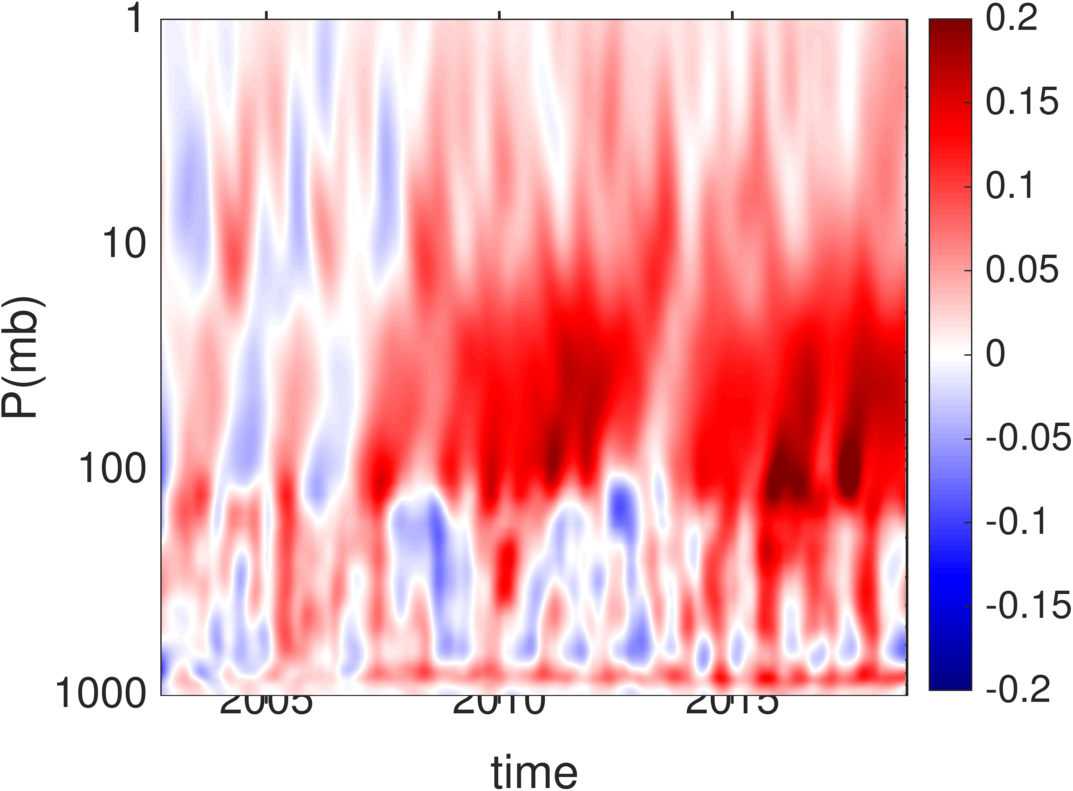
\includegraphics[width=0.9\linewidth]{Figs/CloudAnom/Desc_ocean/ntropics27_era_cld_wv_anom_200209_201808.png}
\end{center}
\end{block}
\end{column}

\begin{column}{0.55\columnwidth}
%\begin{block}{\footnotesize Cloud param rates}
%\begin{block}{\footnotesize UMBC}
%\vspace{-0.1in}
%\begin{center}
%\includegraphics[width=0.95\linewidth]{Figs/CloudAnom/Desc_ocean/ntropic27N_umbc_cld_retr_o%bs_wv_anom_200209_201808.png}
%\end{center}
%\end{block}
\end{column}
\end{columns}

\vspace{-0.45in}

\begin{columns}
\begin{column}{0.55\columnwidth}
\begin{block}{\footnotesize <AK> x ERA}
\vspace{-0.1in}
\begin{center}
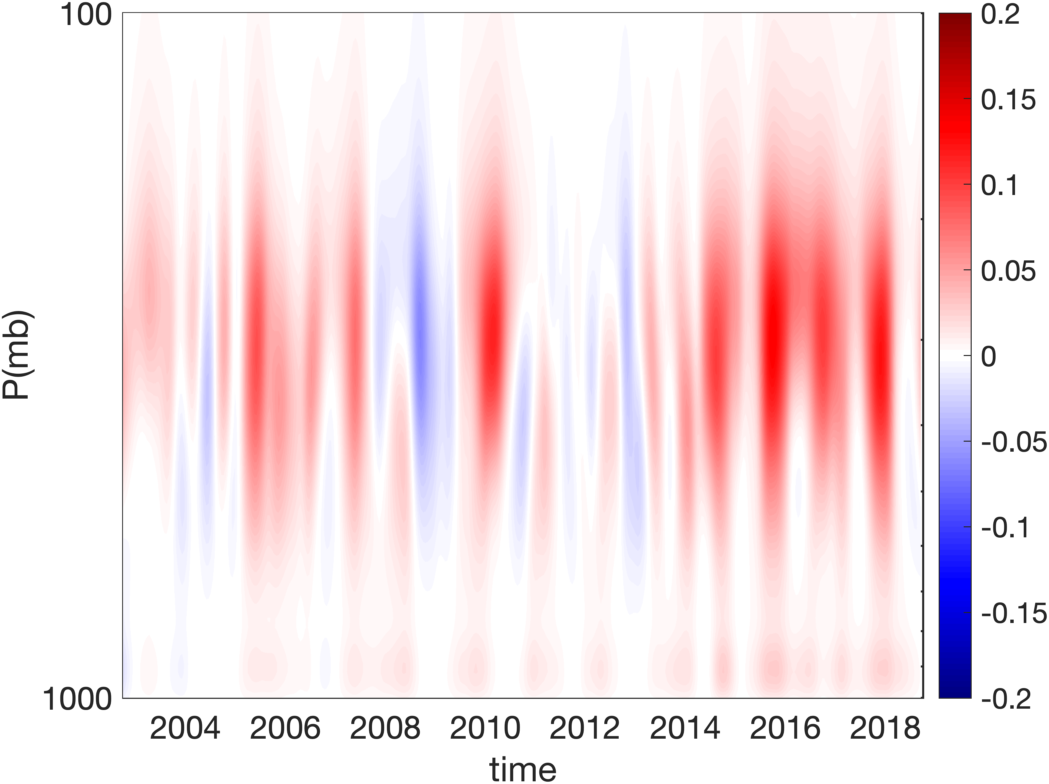
\includegraphics[width=0.95\linewidth]{Figs/CloudAnom/Desc_ocean/ak_x_ntropics27_era_cld_wv_anom_200209_201808.png}
\end{center}
\end{block}
\end{column}

\begin{column}{0.55\columnwidth}
%\begin{block}{\footnotesize Cloud param rates}
\begin{block}{\footnotesize UMBC}
\vspace{-0.1in}
\begin{center}
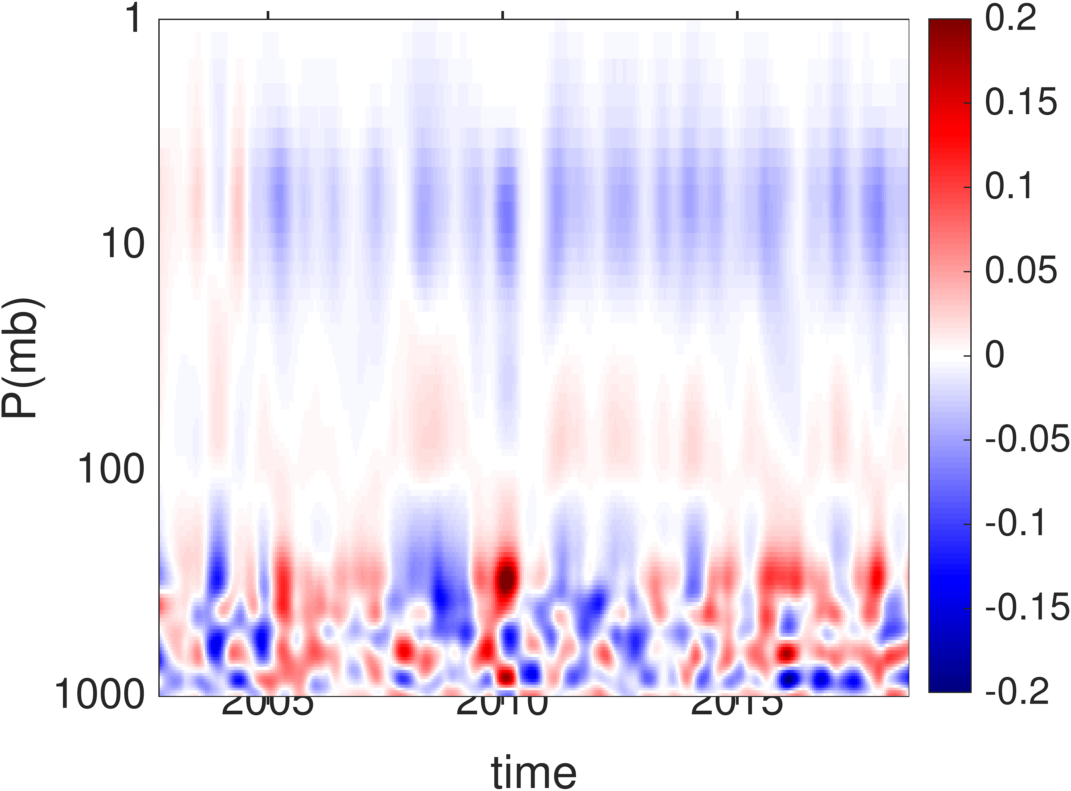
\includegraphics[width=0.95\linewidth]{Figs/CloudAnom/Desc_ocean/ntropic27N_umbc_cld_retr_obs_wv_anom_200209_201808.png}
\end{center}
\end{block}
\end{column}
\end{columns}

\end{frame}

%%%%%%%%%%%%%%%%%%%%%%%%%


\section{Conclusions}
\begin{frame}
  \frametitle{Conclusions}
  \begin{itemize}
  \item Started to work with 16 year AIRS zonally averaged allsky spectra
  \begin{itemize}
    \item too much cloud variability across latitude bins, especially with large 2016 ENSO
    \item at surface difficult to separate low cloud from surface temparature
  \end{itemize}
  \item From allsky spectral rates and anomalies we can get
  \begin{itemize}
    \item  decent trace gas rates; but not from anomalies (so we tie the trace gases to known ``trends'')
    \item using either spectral rates or anomalies, we are obtaining ballpark T/WV/O3 trends
    \item we see recognizable features in anomalies eg QBO in tropical latbins
  \end{itemize}
  \item We will now transition to retrieving gridded anomalies
  \item And, transition to CHIRP radiances once RTA is finishe
  \end{itemize}
\end{frame}

\end{document}

%%%%%%%%%%%%%%%%%%%%%%%%%%%%%%%%%%%%%%%%%%%%%%%%%%%%%%%%%%%%%%%%%%%%%%%%

\section{AllSky LAND/OCEAN}
\subsection{AllSky LAND/OCEAN Rates}

\begin{frame}{Geophysical rates from spectral rates (contd)}
\vspace{-0.3in}

\begin{columns}
\begin{column}{0.55\columnwidth}
\begin{block}{\footnotesize Stemp Rates}
\vspace{-0.1in}
\begin{center}
\includegraphics[width=\linewidth]{Figs/CloudAnom/Desc/stemp_lat_rates_from_obs_specral_rates.pdf}
\end{center}
\footnotesize
This is over ocean only
\end{block}
\end{column}

\begin{column}{0.55\columnwidth}
%\begin{block}{\footnotesize Cloud param rates}
\begin{block}{\footnotesize Trace gas rates}
\vspace{-0.1in}
\begin{center}
%\includegraphics[width=\linewidth]{Figs/CloudAnom/Desc/cloudparam_lat_rates_from_obs_specral_rates.pdf}
\includegraphics[width=\linewidth]{Figs/CloudAnom/Desc/tracegas_lat_rates_from_obs_specral_rates.pdf}
\end{center}
\footnotesize
Preliminary work
\end{block}
\end{column}
\end{columns}
\end{frame}

%%%%%%%%%%

%figure(1);  aslprint_mat('/home/sergio/PAPERS/AIRS/airs_stm_sep19/allsky/Figs/CloudAnom/Desc/wv_lat_p_rates_from_obs_specral_rates',1,1,latx,playsRET,temp_ret*10);
%figure(2);  aslprint_mat('/home/sergio/PAPERS/AIRS/airs_stm_sep19/allsky/Figs/CloudAnom/Desc/tz_lat_p_rates_from_obs_specral_rates',2,1,latx,playsRET,temp_ret*10);
%figure(3);  aslprint_mat('/home/sergio/PAPERS/AIRS/airs_stm_sep19/allsky/Figs/CloudAnom/Desc/o3_lat_p_rates_from_obs_specral_rates',3,1,latx,playsRET,temp_ret*10);
%figure(7);  aslprint('/home/sergio/PAPERS/AIRS/airs_stm_sep19/allsky/Figs/CloudAnom/Desc/tracegas_lat_rates_from_obs_specral_rates.pdf');
%figure(9);  aslprint('/home/sergio/PAPERS/AIRS/airs_stm_sep19/allsky/Figs/CloudAnom/Desc/stemp_lat_rates_from_obs_specral_rates.pdf');
%figure(10); aslprint('/home/sergio/PAPERS/AIRS/airs_stm_sep19/allsky/Figs/CloudAnom/Desc/cloudparam_lat_rates_from_obs_specral_rates.pdf')

\begin{frame}{UMBC AllSky LAND/OCEAN Spectral Rates $\rightarrow$ AllSky Geophysical Rates}
%% see /home/sergio/MATLABCODE/oem_pkg_run/AIRS_new_random_scan_August2019/Plotutils/plot_all_latbins_fewlays.m
%% see /home/sergio/MATLABCODE/oem_pkg_run_sergio_AuxJacs/MakeProfs/plot_anomalies.m
\vspace{-0.35in}

\begin{columns}
\begin{column}{0.45\columnwidth}
\begin{block}{\footnotesize dT(z,t)/dt}
\vspace{-0.1in}
\begin{center}
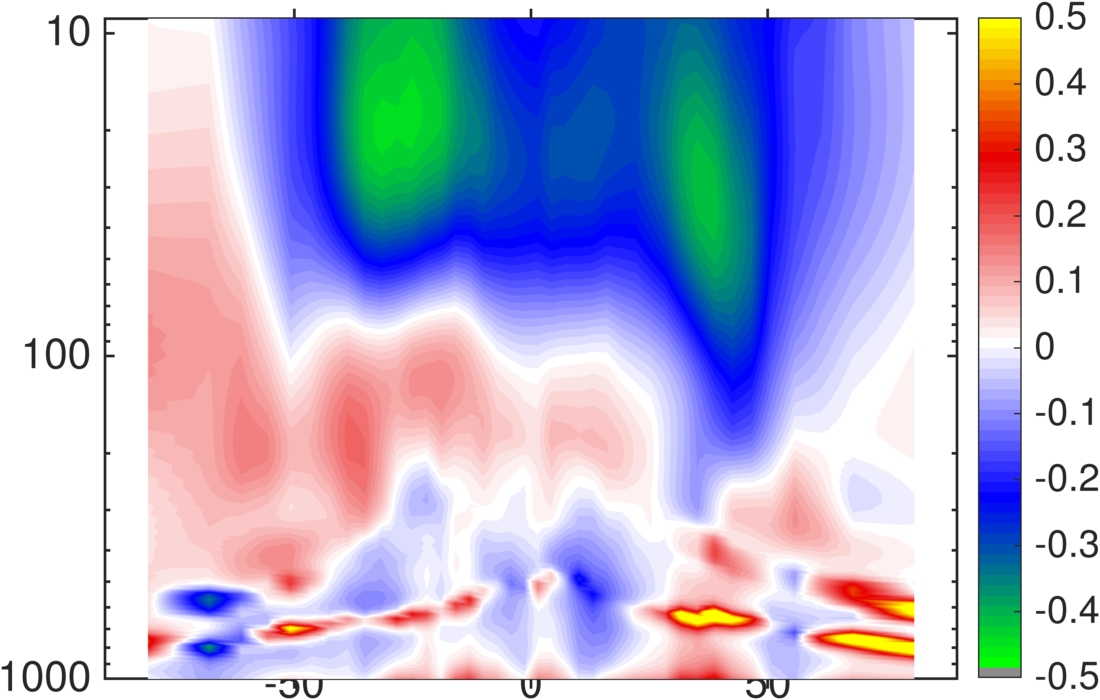
\includegraphics[width=\linewidth]{Figs/CloudAnom/Desc/tz_lat_p_rates_from_obs_specral_rates.png}
\end{center}
\end{block}
\end{column}

\begin{column}{0.45\columnwidth}
\begin{block}{\footnotesize $frac$ dWV(z,t)/dt}
\vspace{-0.1in}
\begin{center}
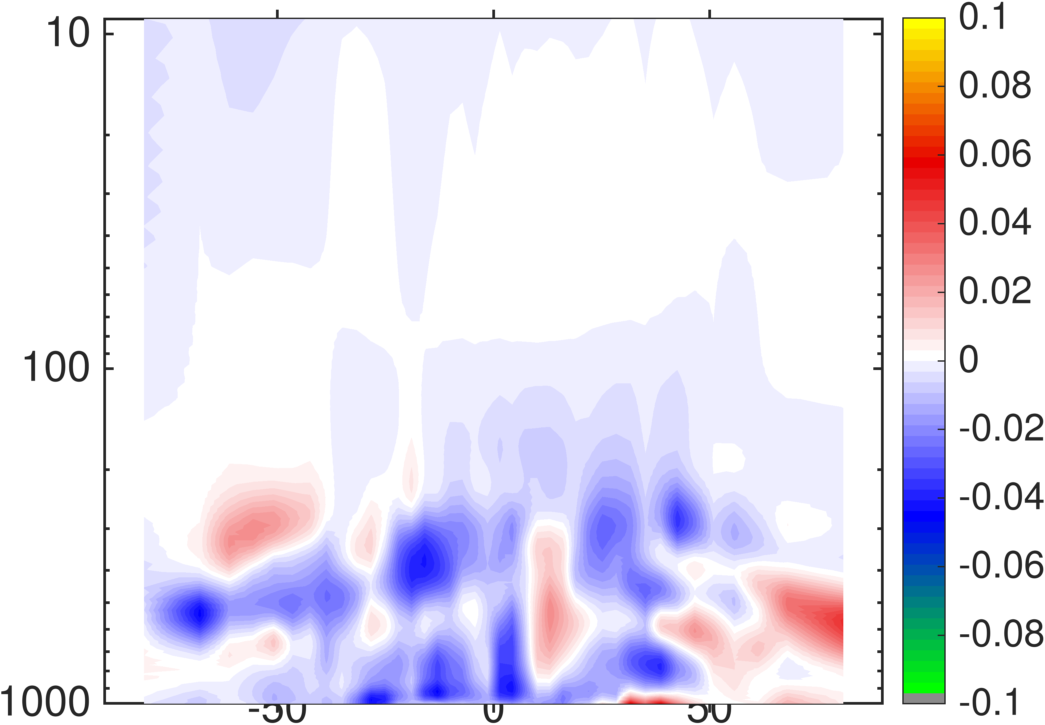
\includegraphics[width=\linewidth]{Figs/CloudAnom/Desc/wv_lat_p_rates_from_obs_specral_rates.png}
\end{center}
\end{block}
\end{column}
\end{columns}

\vspace{-0.25in}

\begin{columns}
\begin{column}{0.45\columnwidth}
\begin{block}{\footnotesize $frac$ dO3(z,t)/dt}
\vspace{-0.1in}
\begin{center}
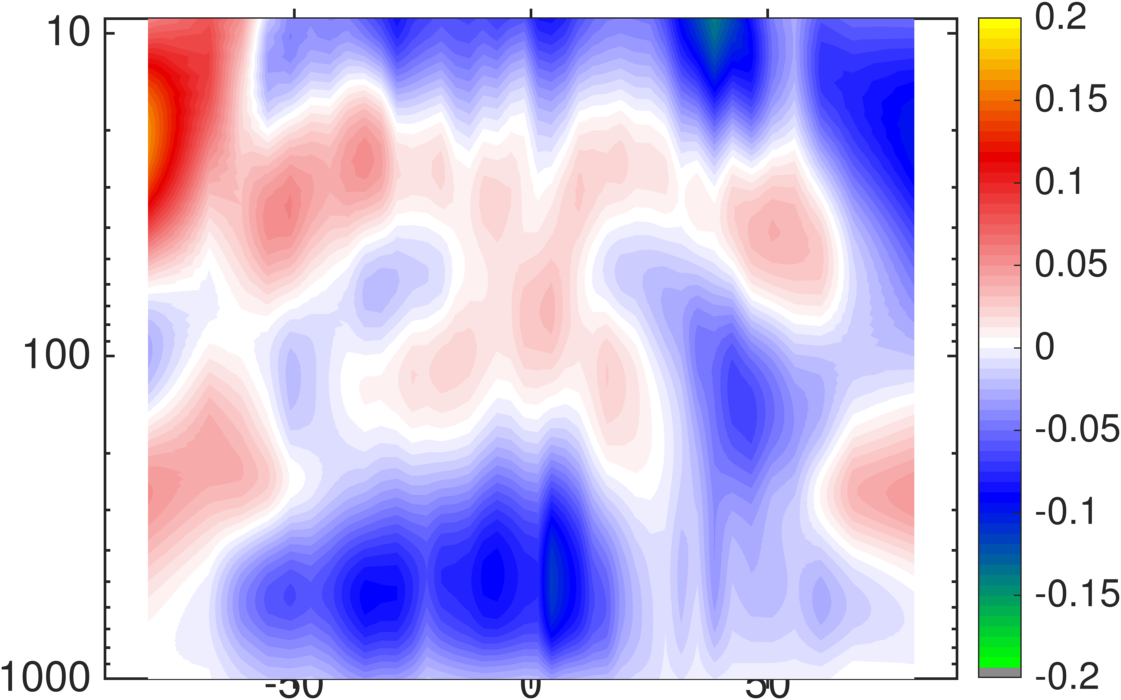
\includegraphics[width=\linewidth]{Figs/CloudAnom/Desc/o3_lat_p_rates_from_obs_specral_rates.png}
\end{center}
\end{block}
\end{column}

\begin{column}{0.45\columnwidth}
%\begin{block}{\footnotesize Another Small Title}
%\vspace{-0.1in}
%\begin{center}
%\includegraphics[width=\linewidth]{{Figs/CloudAnom/umbc_clr_retr_obs_stemp_rate_200209_201808.png}
%\end{center}
%\end{block}

\end{column}
\end{columns}
\end{frame}

%%%%%

\begin{frame}{ERA AllSky LAND/OCEAN Rates $\rightarrow$ AllSky AK $\times$ Rates}
%% see /home/sergio/MATLABCODE/oem_pkg_run/AIRS_new_random_scan_August2019/Plotutils/compute_geo_rates_ak_fewlays.m}
%% see /home/sergio/MATLABCODE/oem_pkg_run_sergio_AuxJacs/MakeProfs/plot_anomalies.m
\vspace{-0.35in}

\begin{columns}
\begin{column}{0.45\columnwidth}
\begin{block}{\footnotesize dT(z,t)/dt}
\vspace{-0.1in}
\begin{center}
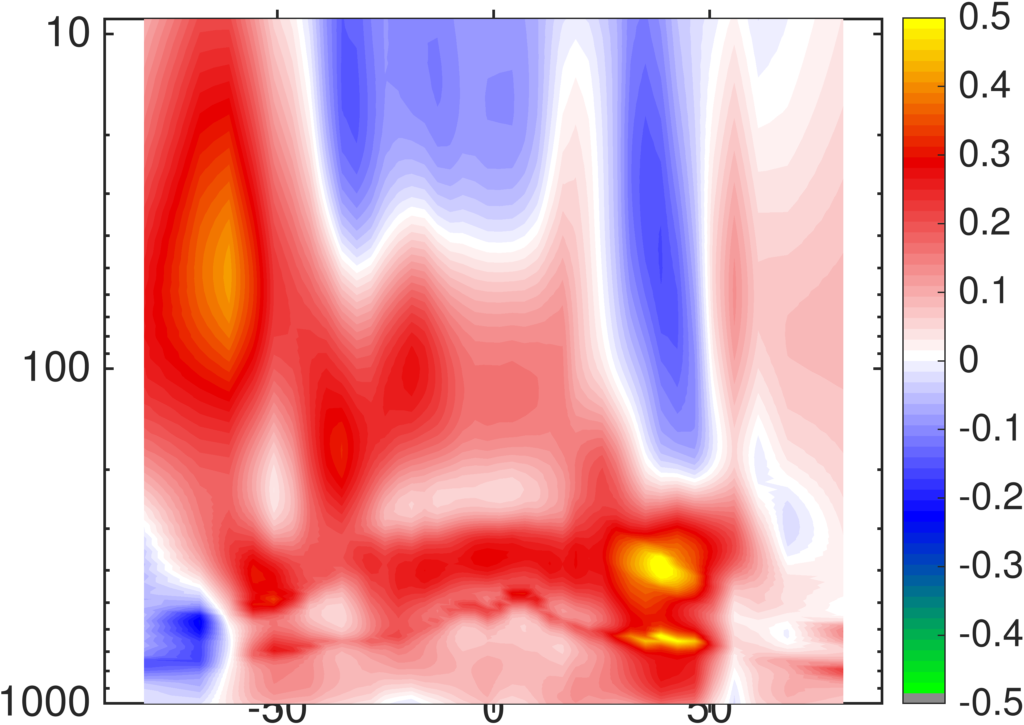
\includegraphics[width=\linewidth]{Figs/CloudAnom/Desc/ak_x_ERAtzrates.png}
\end{center}
\end{block}
\end{column}

\begin{column}{0.45\columnwidth}
\begin{block}{\footnotesize $frac$ dWV(z,t)/dt}
\vspace{-0.1in}
\begin{center}
\includegraphics[width=\linewidth]{Figs/CloudAnom/Desc/ak_x_ERAwvrates.png}
\end{center}
\end{block}
\end{column}
\end{columns}

\vspace{-0.25in}

\begin{columns}
\begin{column}{0.45\columnwidth}
\begin{block}{\footnotesize $frac$ dO3(z,t)/dt}
\vspace{-0.1in}
\begin{center}
\includegraphics[width=\linewidth]{Figs/CloudAnom/Desc/ak_x_ERAo3rates.png}
\end{center}
\end{block}
\end{column}

\begin{column}{0.45\columnwidth}
%\begin{block}{\footnotesize Another Small Title}
%\vspace{-0.1in}
%\begin{center}
%\includegraphics[width=\linewidth]{{Figs/CloudAnom/umbc_clr_retr_obs_stemp_rate_200209_201808.png}
%\end{center}
%\end{block}

\end{column}
\end{columns}
\end{frame}

%%%%%

\begin{frame}{27 N AllSky Land/Ocean Retrieved Geophysical Anomalies}
%% see /home/sergio/MATLABCODE/oem_pkg_run_sergio_AuxJacs/MakeProfs/plot_anomalies.m
\vspace{-0.35in}

GAH
\begin{columns}
\begin{column}{0.45\columnwidth}
\begin{block}{\footnotesize T(z,t)}
\vspace{-0.1in}
\begin{center}
\includegraphics[width=\linewidth]{Figs/CloudAnom/Desc/ntropic27N_umbc_cld_retr_obs_ptemp_anom_200209_201808.png}
\end{center}
\end{block}
\end{column}

\begin{column}{0.45\columnwidth}
\begin{block}{\footnotesize $frac$ WV(z,t)}
\vspace{-0.1in}
\begin{center}
\includegraphics[width=\linewidth]{Figs/CloudAnom/Desc/ntropic27N_umbc_cld_retr_obs_wv_anom_200209_201808.png}
\end{center}
\end{block}
\end{column}
\end{columns}

\vspace{-0.25in}

\begin{columns}
\begin{column}{0.45\columnwidth}
\begin{block}{\footnotesize $frac$ O3(z,t)}
\vspace{-0.1in}
\begin{center}
\includegraphics[width=\linewidth]{Figs/CloudAnom/Desc/ntropic27N_umbc_cld_retr_obs_o3_anom_200209_201808.png}
\end{center}
\end{block}
\end{column}

\begin{column}{0.45\columnwidth}
%\begin{block}{\footnotesize Another Small Title}
%\vspace{-0.1in}
%\begin{center}
%\includegraphics[width=\linewidth]{{Figs/CloudAnom/era_cld_stemp_anom_200209_201808.png}
%\end{center}
%\end{block}

\end{column}
\end{columns}
\end{frame}

%%%%%

%%% Local Variables:
%%% mode: latex
%%% TeX-master: t
%%% End:
